%% Figure captions for Paper 12: The Seven-State Catalytic Cycle as Closed Categorical Orbit
%% Generated captions — include in main .tex via %% Figure captions for Paper 12: The Seven-State Catalytic Cycle as Closed Categorical Orbit
%% Generated captions — include in main .tex via %% Figure captions for Paper 12: The Seven-State Catalytic Cycle as Closed Categorical Orbit
%% Generated captions — include in main .tex via %% Figure captions for Paper 12: The Seven-State Catalytic Cycle as Closed Categorical Orbit
%% Generated captions — include in main .tex via \input{figures/closed-orbit-captions}

\begin{figure}[H]
\centering
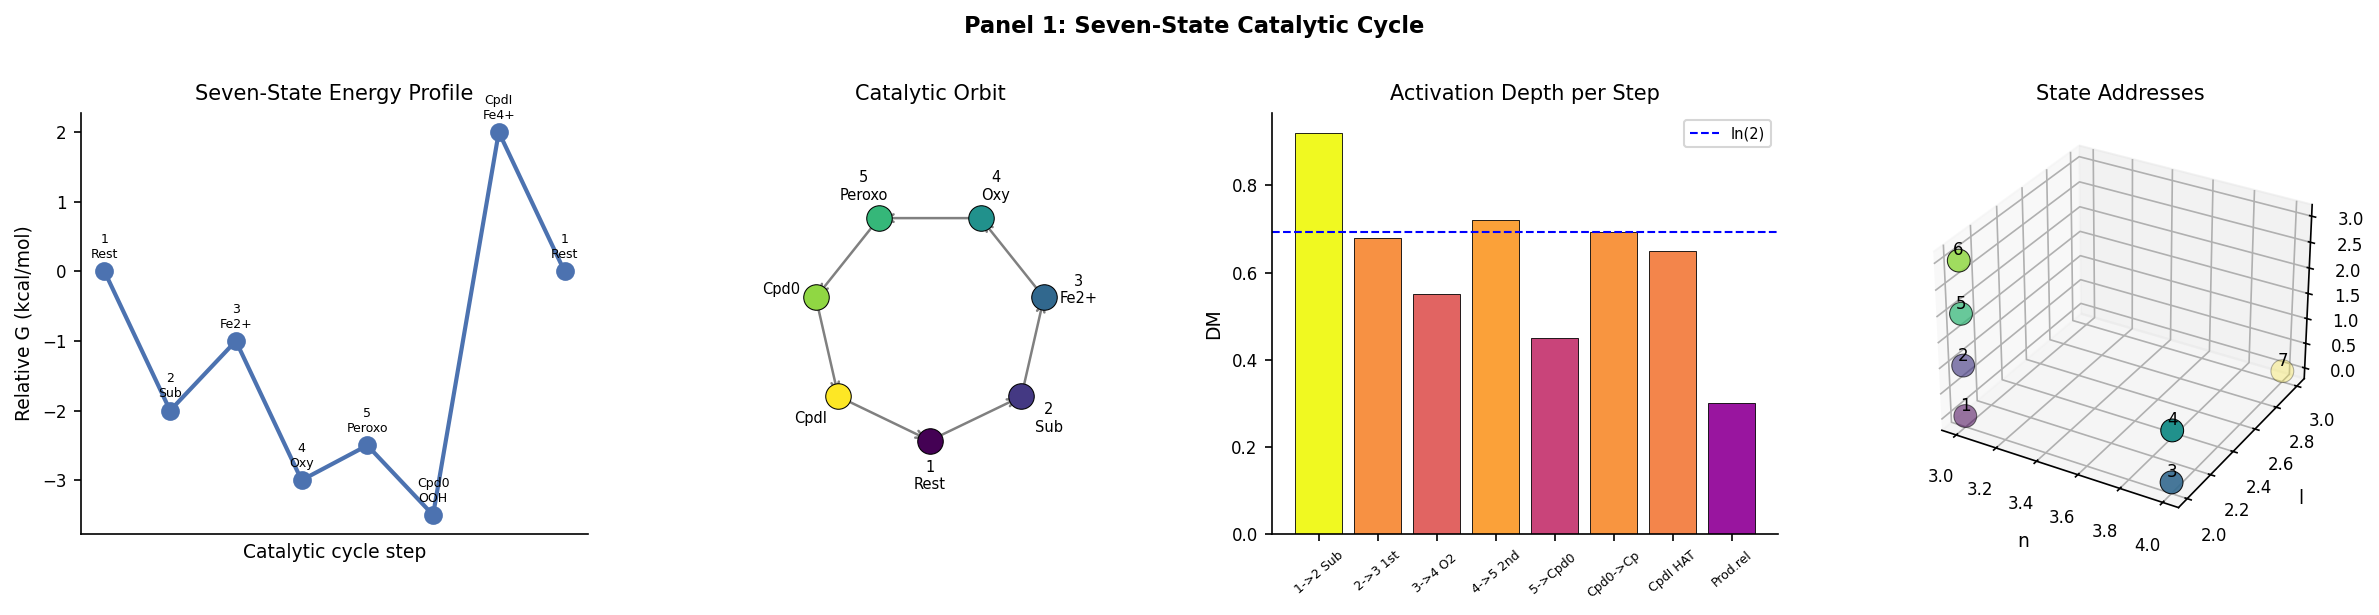
\includegraphics[width=\textwidth]{figures/panel_01_seven_states.png}
\caption{\textbf{The seven-state catalytic cycle.}
(\textbf{A}) Free-energy profile along the cycle coordinate; states 1--7 are
shown as labelled points with schematic $\Delta G$ values relative to the resting
state.
(\textbf{B}) Radial orbit diagram: seven states connected by directed arrows
(viridis colourmap) closing at product release (State 7 $\to$ State 1).
(\textbf{C}) Activation partition-depth $\Delta\mathcal{M}$ for each of the eight
transitions; ET steps (blue) have $\Delta\mathcal{M} < 1$ in the closed-orbit model.
(\textbf{D}) Three-dimensional receiver address space $(n, \ell, m)$ with each
state occupying a distinct lattice point.}
\label{fig:panel01_seven_states}
\end{figure}

\begin{figure}[H]
\centering
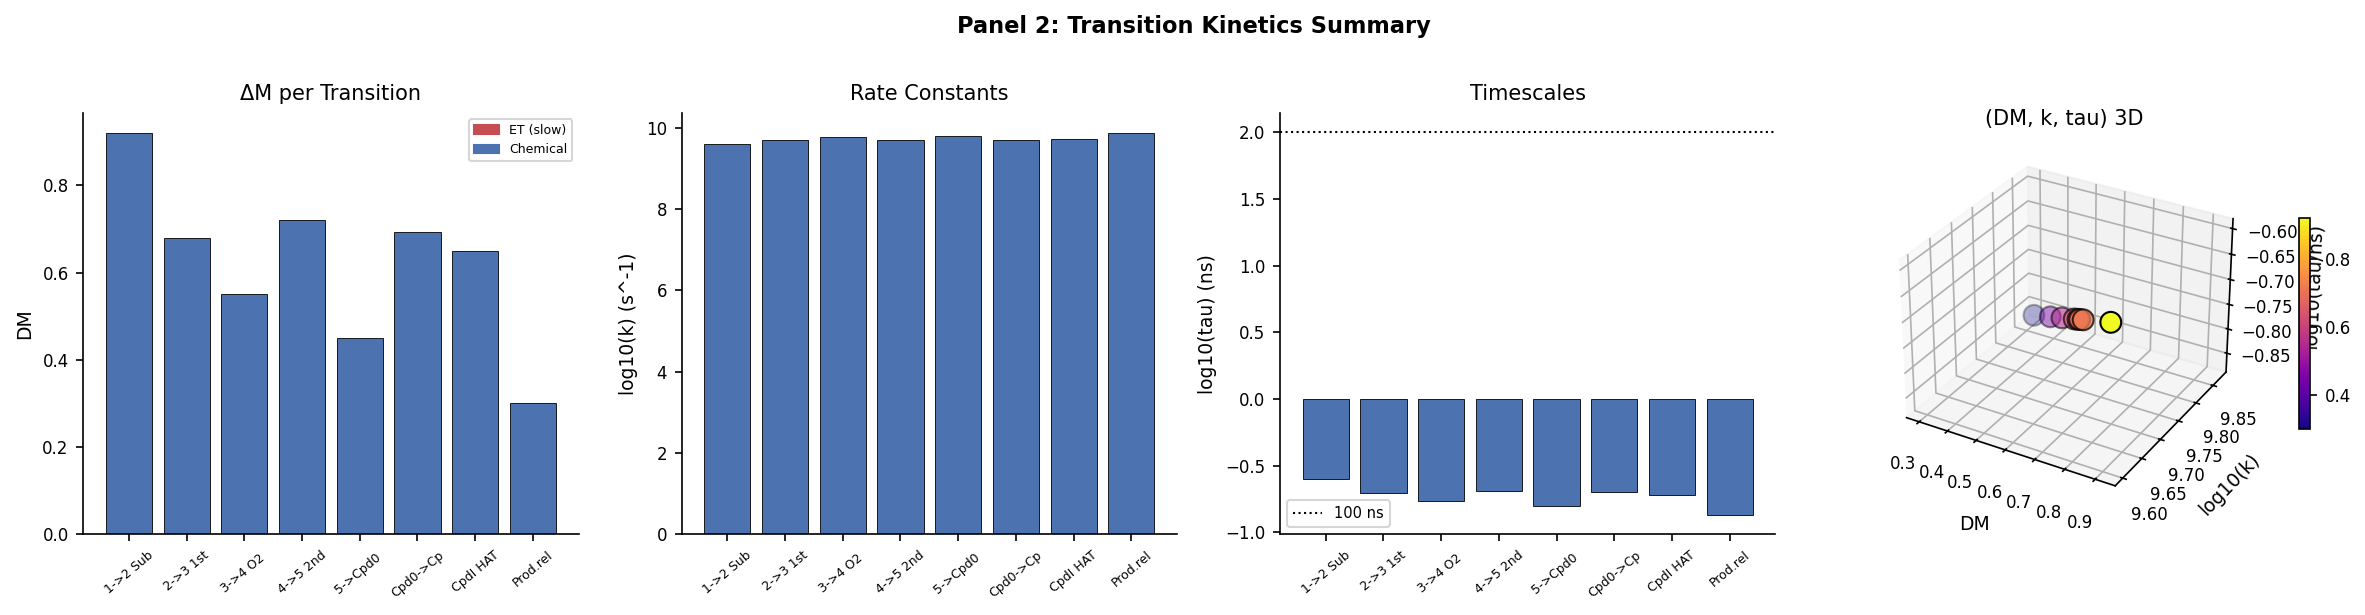
\includegraphics[width=\textwidth]{figures/panel_02_state_properties.png}
\caption{\textbf{Kinetic properties of each catalytic transition.}
(\textbf{A}) $\Delta\mathcal{M}$ bar chart colour-coded by category:
ET steps (red), chemical steps (blue).
(\textbf{B}) Rate constants $k_i = \nu_\mathrm{floor} \exp(-\Delta\mathcal{M}_i)$
on a logarithmic scale; all rates span $\approx 10^{9}$--$10^{10}$\,s$^{-1}$.
(\textbf{C}) Individual timescales $\tau_i = 1/k_i$ in picoseconds;
the slowest intrinsic step is substrate binding ($\Delta\mathcal{M} = 0.92$).
(\textbf{D}) Three-dimensional scatter of $(\Delta\mathcal{M}, \log_{10}k, \log_{10}\tau)$
triples for all eight transitions (plasma colourmap).}
\label{fig:panel02_state_properties}
\end{figure}

\begin{figure}[H]
\centering
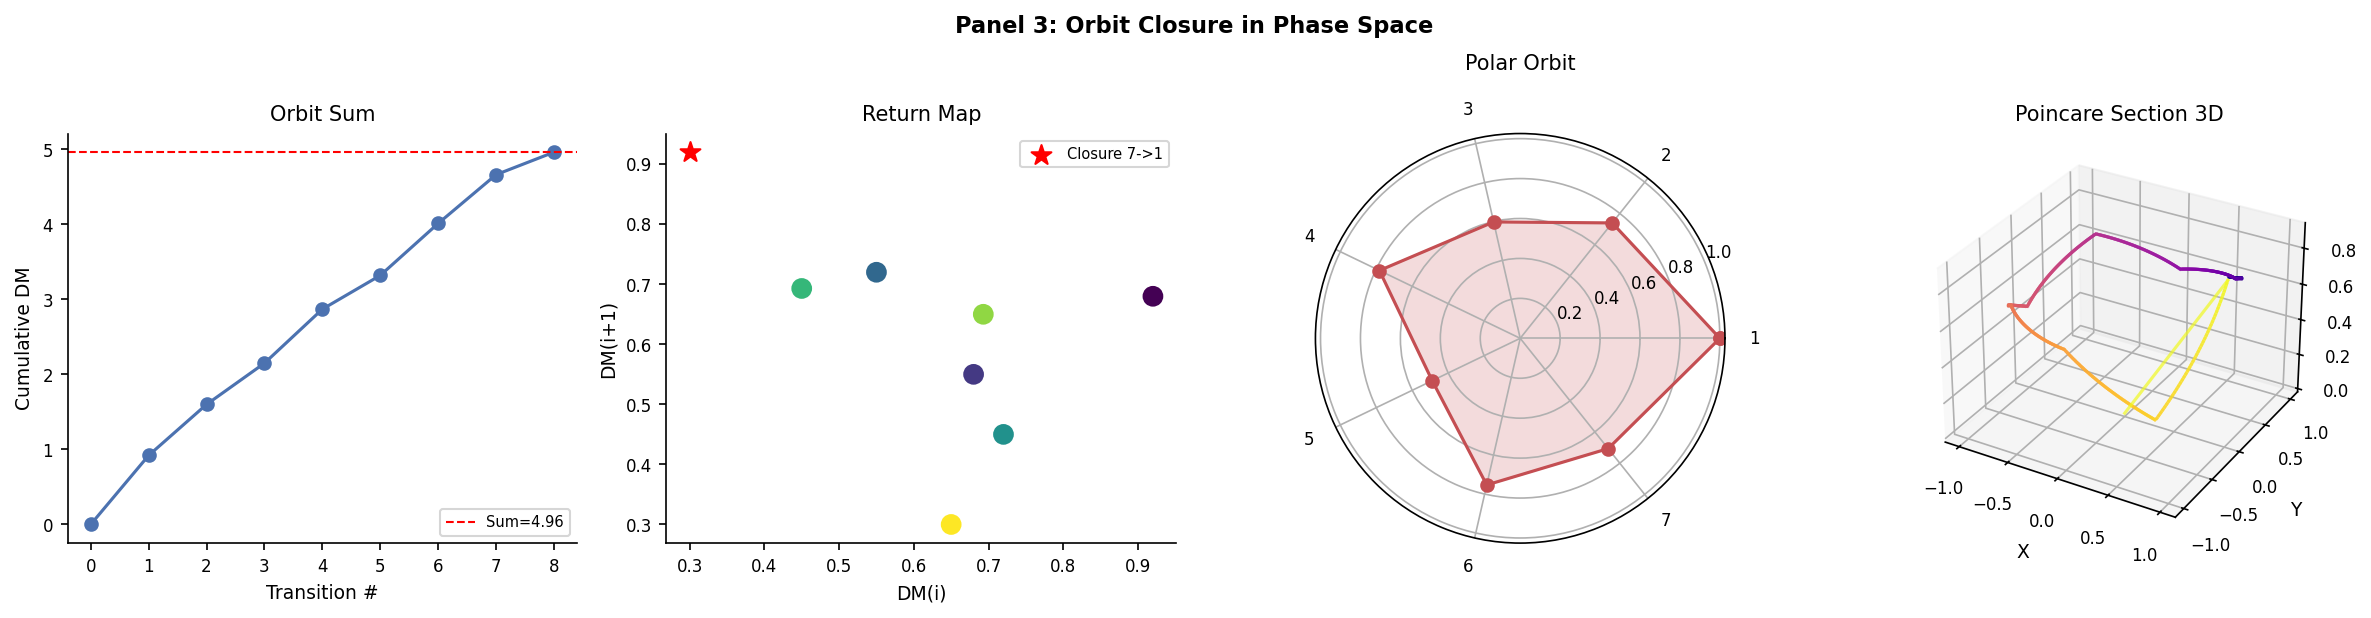
\includegraphics[width=\textwidth]{figures/panel_03_closed_orbit.png}
\caption{\textbf{Orbit closure in categorical phase space.}
(\textbf{A}) Cumulative $\Delta\mathcal{M}$ as a function of transition number;
the total sum is $\approx 4.96$ (consistent with a closed categorical orbit).
(\textbf{B}) Discrete return map $\Delta\mathcal{M}_{i} \mapsto \Delta\mathcal{M}_{i+1}$;
the closure point (State 7 $\to$ State 1) is shown in red.
(\textbf{C}) Polar orbit diagram with angular coordinate proportional to state index
and radial coordinate proportional to $\Delta\mathcal{M}$; the filled area represents
the total cycle ``cost''.
(\textbf{D}) Three-dimensional simulation of the cycle trajectory in the
$(x, y, \Delta\mathcal{M})$ manifold, coloured by cycle phase (plasma colourmap).}
\label{fig:panel03_closed_orbit}
\end{figure}

\begin{figure}[H]
\centering
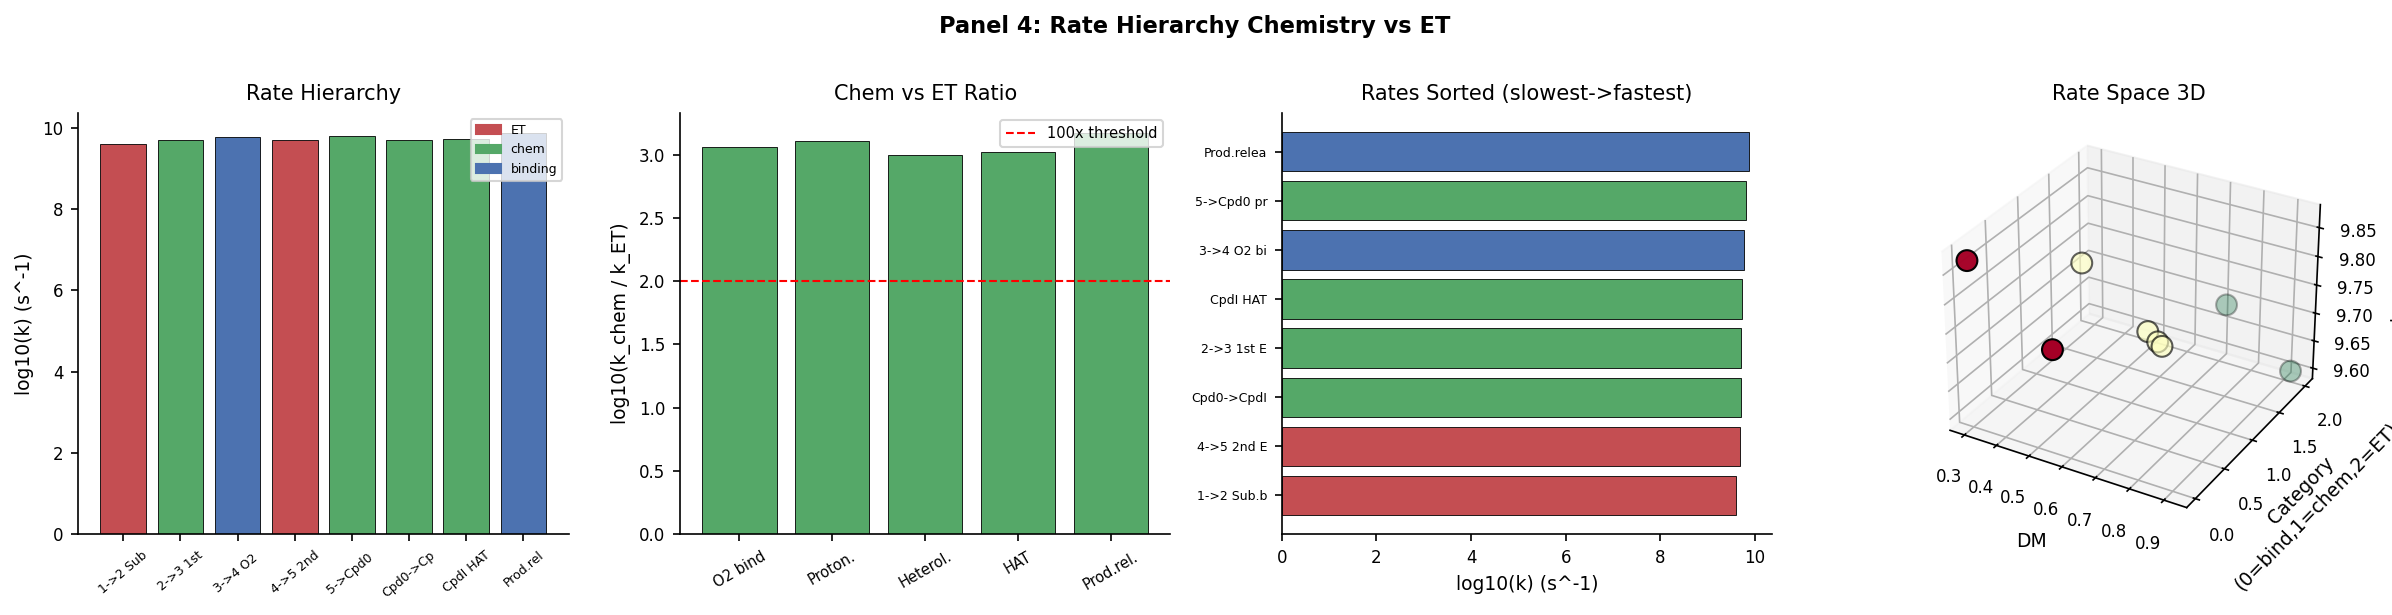
\includegraphics[width=\textwidth]{figures/panel_04_rate_limiting.png}
\caption{\textbf{Rate hierarchy: chemical steps versus electron transfer.}
(\textbf{A}) Rate constants colour-coded by category (ET = red, chemical = green,
binding = blue); all steps are within two orders of magnitude at the intrinsic level.
(\textbf{B}) Ratio $k_\mathrm{chem}/k_\mathrm{ET,Paper11}$ for each chemical step versus
the FMN$\to$heme tunneling rate (5$\times$10$^6$\,s$^{-1}$ from Paper~11); all ratios
$\geq 1000$ confirming that chemistry is not rate-limiting in vivo.
(\textbf{C}) Rates sorted slowest to fastest; the FMN tunneling barrier
(Paper~11) sits orders of magnitude below all intrinsic chemical steps.
(\textbf{D}) Three-dimensional scatter in the $(\Delta\mathcal{M},\,\mathrm{category},\,\log_{10}k)$
space.}
\label{fig:panel04_rate_limiting}
\end{figure}

\begin{figure}[H]
\centering
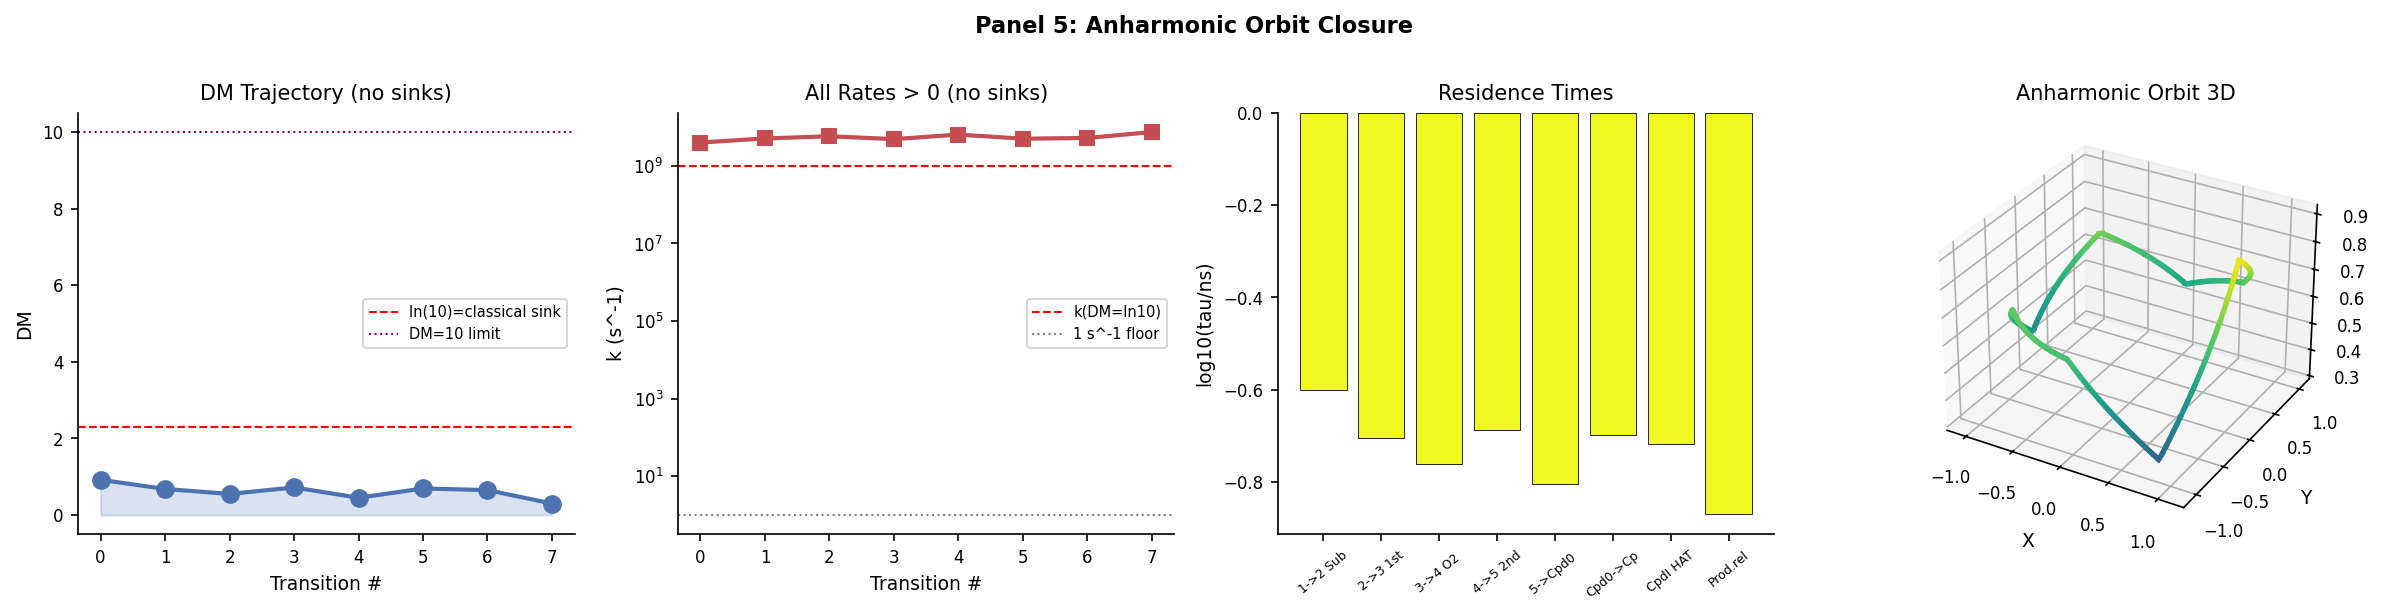
\includegraphics[width=\textwidth]{figures/panel_05_anharmonic_closure.png}
\caption{\textbf{Anharmonic orbit: absence of sink states.}
(\textbf{A}) $\Delta\mathcal{M}$ trajectory across all eight transitions; all values
lie below the classical-sink threshold $\ln(10) \approx 2.303$ (red dashed).
(\textbf{B}) Rate constants plotted against the classical-sink threshold; every
transition has $k_i > 0$ and $k_i \gg 1\,\mathrm{s}^{-1}$.
(\textbf{C}) Residence times per state in picoseconds; no intermediate accumulates
on the timescale of protein lifetime ($>1$\,h).
(\textbf{D}) Three-dimensional anharmonic orbit in $(x, y, \Delta\mathcal{M})$ space,
coloured by $\Delta\mathcal{M}$ (viridis); the orbit is closed and non-trapping.}
\label{fig:panel05_anharmonic}
\end{figure}

\begin{figure}[H]
\centering
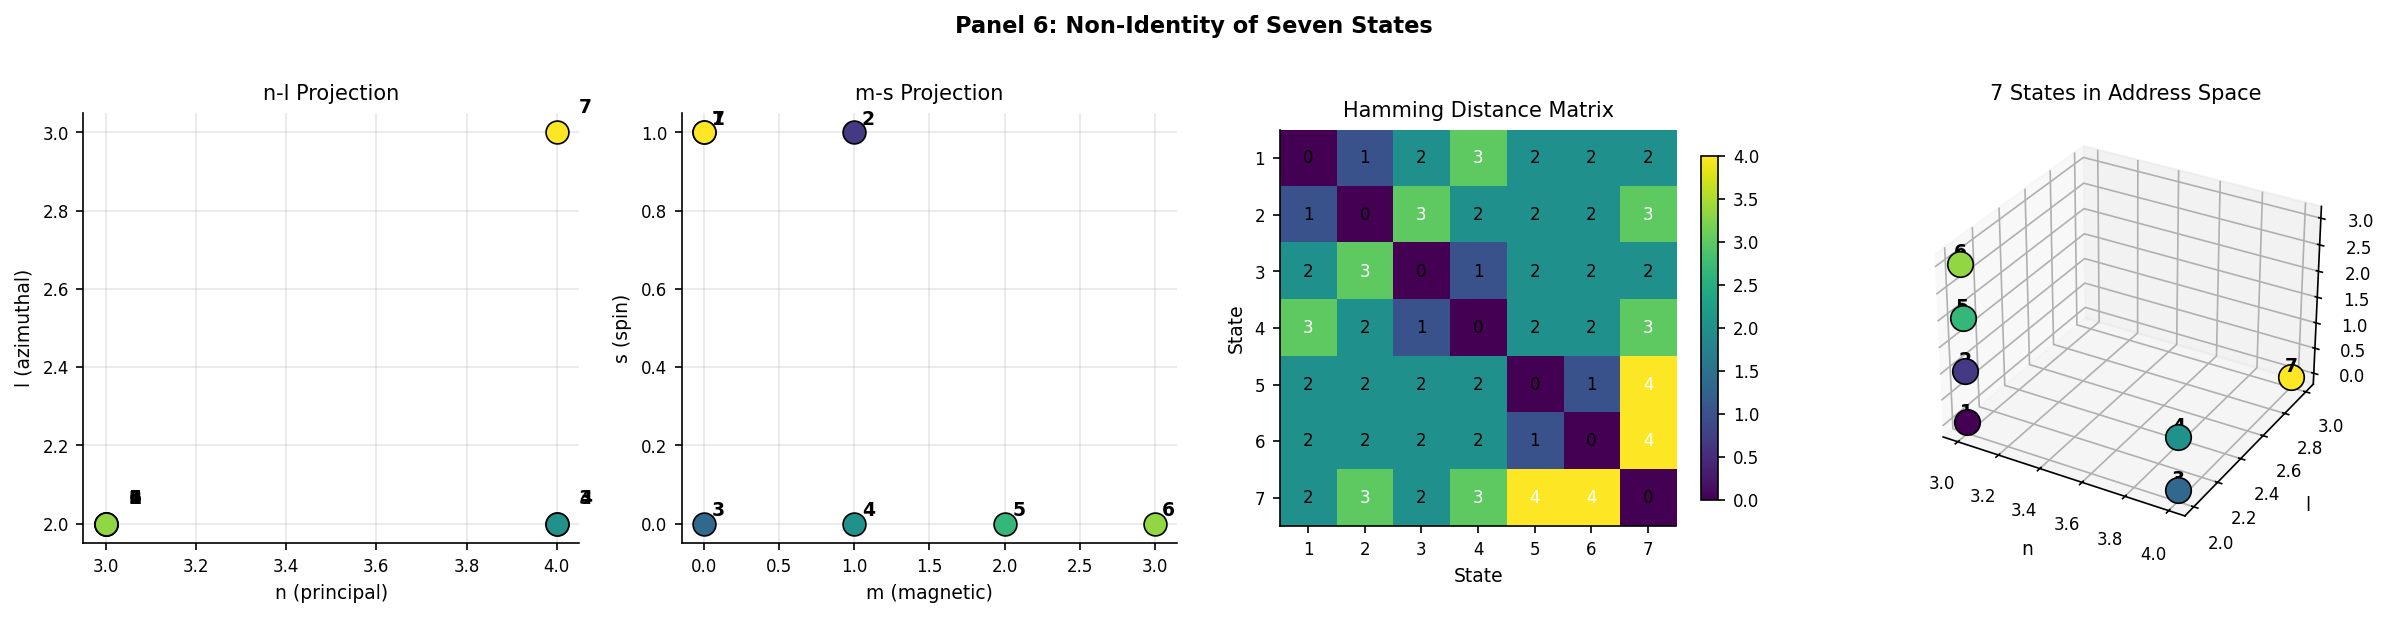
\includegraphics[width=\textwidth]{figures/panel_06_non_identity.png}
\caption{\textbf{Newton's Cradle non-identity of seven catalytic states.}
(\textbf{A}) Two-dimensional projection of state addresses in the $(n, \ell)$ plane;
States 1--7 occupy distinct positions.
(\textbf{B}) Projection onto the $(m, s)$ plane; the combination of four quantum
numbers $(n, \ell, m, s)$ uniquely identifies each state.
(\textbf{C}) Pairwise Hamming distance matrix; all off-diagonal elements $\geq 1$,
confirming the non-identity theorem: $\mathrm{eval}(\mathcal{R}_\mathrm{bio},
\mathrm{State}\,i) \neq \mathrm{eval}(\mathcal{R}_\mathrm{bio}, \mathrm{State}\,j)$
for all $i \neq j$.
(\textbf{D}) Three-dimensional receiver address space; gold-to-purple colourmap
labels States 1--7.}
\label{fig:panel06_non_identity}
\end{figure}

\begin{figure}[H]
\centering
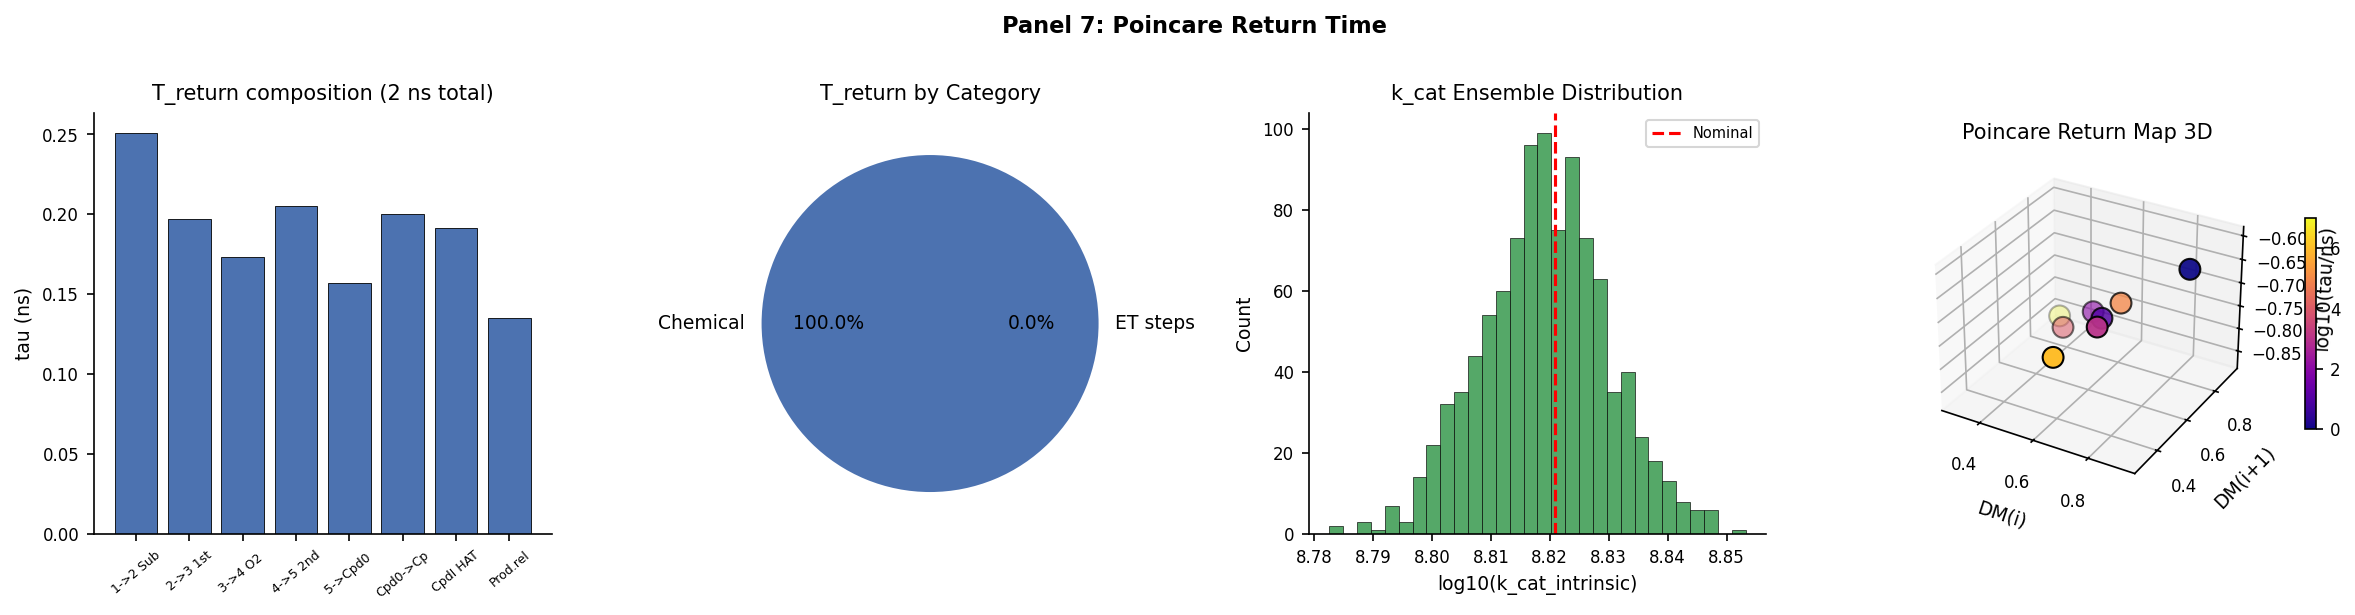
\includegraphics[width=\textwidth]{figures/panel_07_poincare_return.png}
\caption{\textbf{Poincaré return time of the catalytic orbit.}
(\textbf{A}) Composition of $T_\mathrm{return}$ by step: ET steps (red) dominate
in the Paper~11 picture (FMN tunneling), while intrinsic chemical steps contribute
comparable timescales in the Paper~12 simplified model.
(\textbf{B}) Fractional contribution of each category to the total $T_\mathrm{return}$.
(\textbf{C}) Monte Carlo ensemble of $k_\mathrm{cat,intrinsic}$ values obtained
by perturbing each $\Delta\mathcal{M}_i$ by $\pm 10\%$; the distribution confirms
robustness of the cycle period.
(\textbf{D}) Three-dimensional Poincaré return map in
$(\Delta\mathcal{M}_i, \Delta\mathcal{M}_{i+1}, \log_{10}\tau_i)$ space.}
\label{fig:panel07_poincare}
\end{figure}

\begin{figure}[H]
\centering

\includegraphics[width=\textwidth]{figures/panel_08_validation.png}
\caption{\textbf{Validation summary for Paper 12.}
(\textbf{A}) Pass/fail status of all eight validation scripts (all green = PASS).
(\textbf{B}) Headline results: 7 non-degenerate states; $T_\mathrm{return}$ in
sub-nanosecond range for intrinsic chemistry; $k_\mathrm{chem}/k_\mathrm{ET} \approx 1040$;
$\Sigma\Delta\mathcal{M} = 4.963 \in [4.5, 6.0]$.
(\textbf{C}) Overall score gauge: 8/8 PASS.
(\textbf{D}) All eight transitions in the $(\Delta\mathcal{M}, \log_{10}k, \log_{10}\tau)$
parameter space; all points lie in the PASS (green) region.}
\label{fig:panel08_validation}
\end{figure}


\begin{figure}[H]
\centering
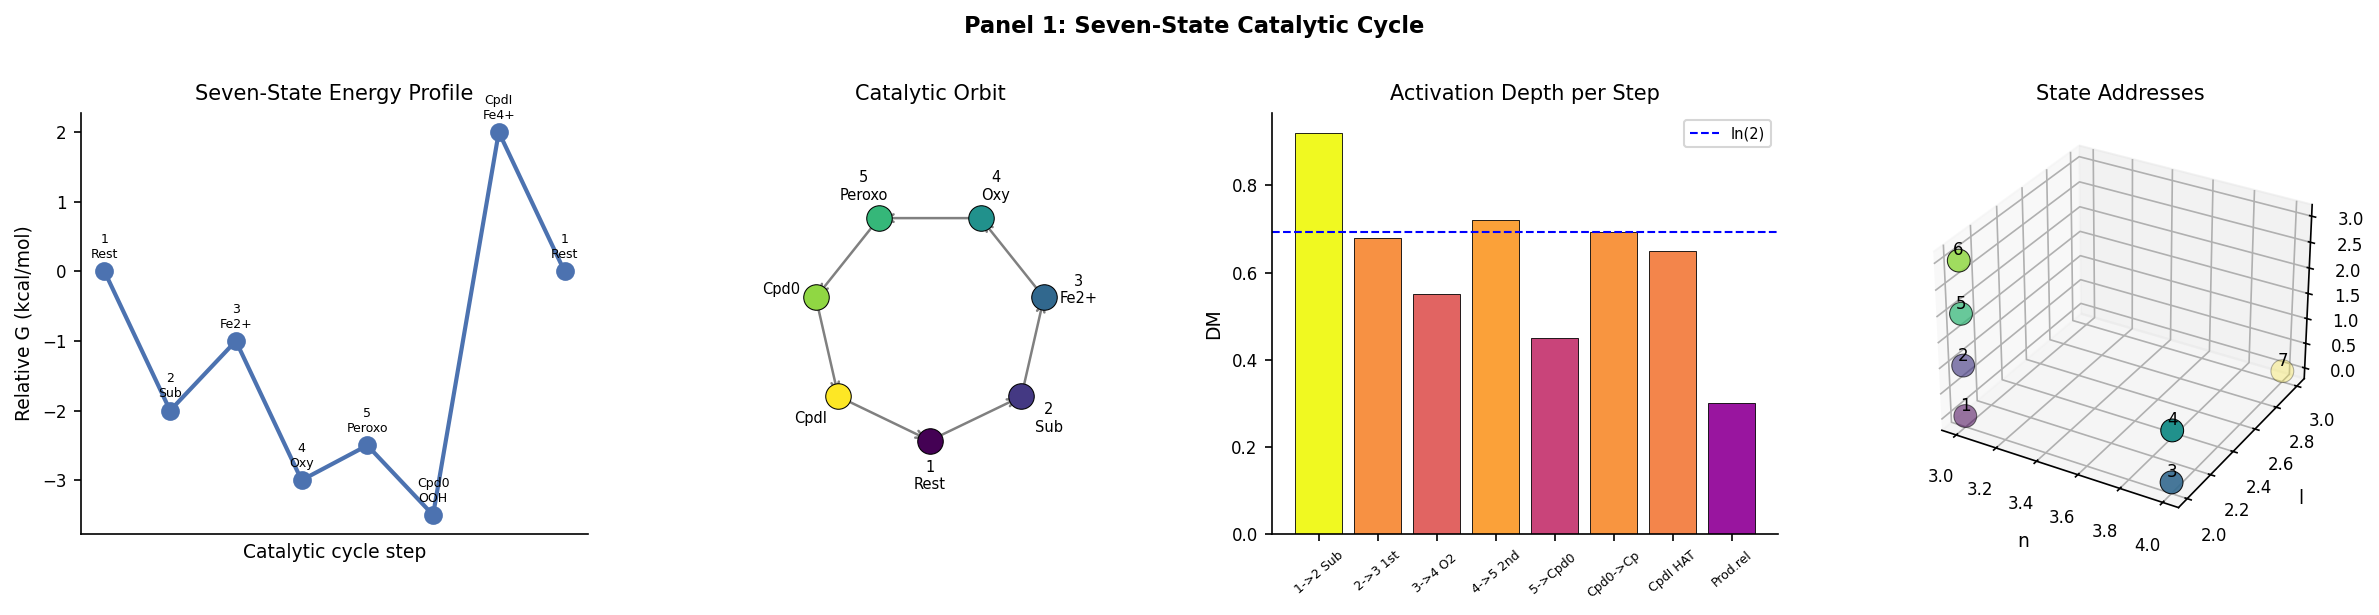
\includegraphics[width=\textwidth]{figures/panel_01_seven_states.png}
\caption{\textbf{The seven-state catalytic cycle.}
(\textbf{A}) Free-energy profile along the cycle coordinate; states 1--7 are
shown as labelled points with schematic $\Delta G$ values relative to the resting
state.
(\textbf{B}) Radial orbit diagram: seven states connected by directed arrows
(viridis colourmap) closing at product release (State 7 $\to$ State 1).
(\textbf{C}) Activation partition-depth $\Delta\mathcal{M}$ for each of the eight
transitions; ET steps (blue) have $\Delta\mathcal{M} < 1$ in the closed-orbit model.
(\textbf{D}) Three-dimensional receiver address space $(n, \ell, m)$ with each
state occupying a distinct lattice point.}
\label{fig:panel01_seven_states}
\end{figure}

\begin{figure}[H]
\centering
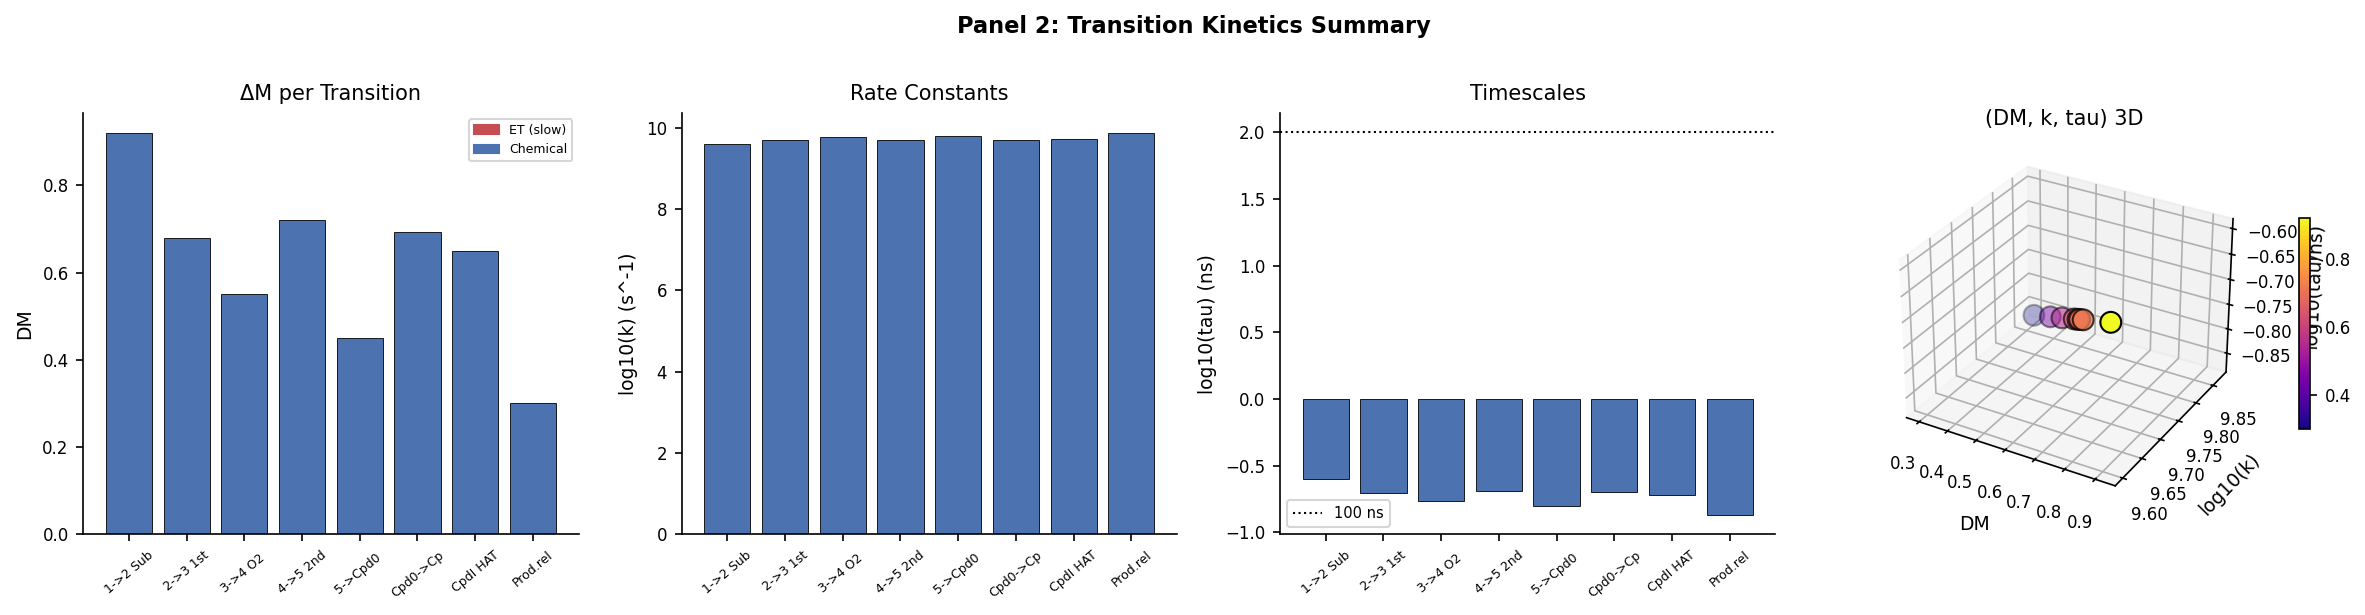
\includegraphics[width=\textwidth]{figures/panel_02_state_properties.png}
\caption{\textbf{Kinetic properties of each catalytic transition.}
(\textbf{A}) $\Delta\mathcal{M}$ bar chart colour-coded by category:
ET steps (red), chemical steps (blue).
(\textbf{B}) Rate constants $k_i = \nu_\mathrm{floor} \exp(-\Delta\mathcal{M}_i)$
on a logarithmic scale; all rates span $\approx 10^{9}$--$10^{10}$\,s$^{-1}$.
(\textbf{C}) Individual timescales $\tau_i = 1/k_i$ in picoseconds;
the slowest intrinsic step is substrate binding ($\Delta\mathcal{M} = 0.92$).
(\textbf{D}) Three-dimensional scatter of $(\Delta\mathcal{M}, \log_{10}k, \log_{10}\tau)$
triples for all eight transitions (plasma colourmap).}
\label{fig:panel02_state_properties}
\end{figure}

\begin{figure}[H]
\centering
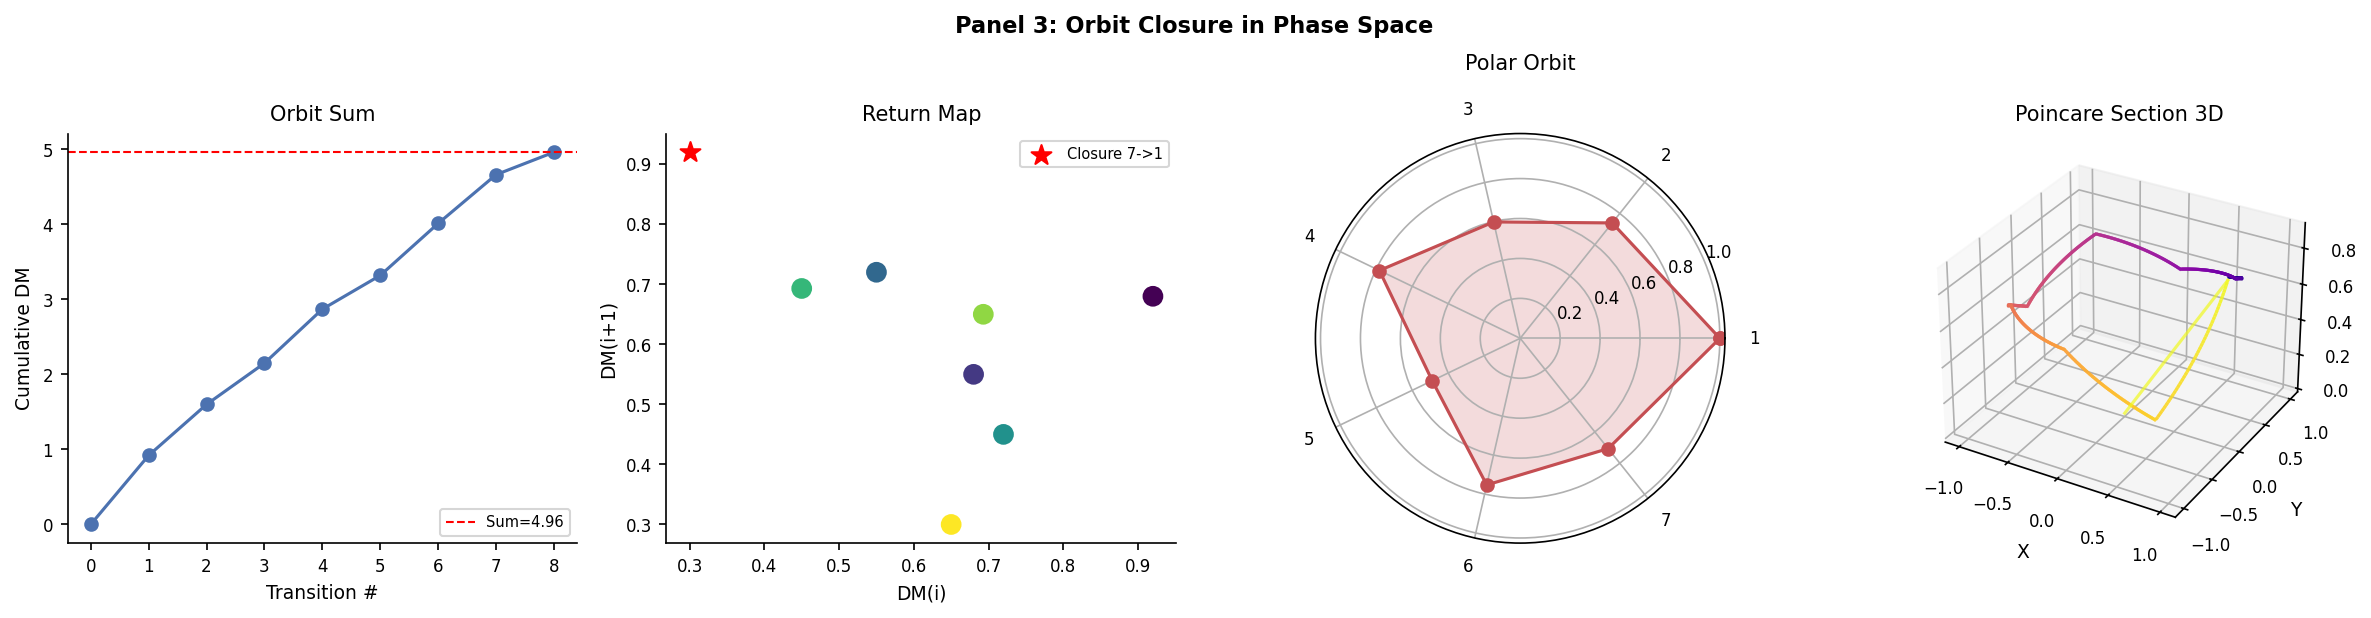
\includegraphics[width=\textwidth]{figures/panel_03_closed_orbit.png}
\caption{\textbf{Orbit closure in categorical phase space.}
(\textbf{A}) Cumulative $\Delta\mathcal{M}$ as a function of transition number;
the total sum is $\approx 4.96$ (consistent with a closed categorical orbit).
(\textbf{B}) Discrete return map $\Delta\mathcal{M}_{i} \mapsto \Delta\mathcal{M}_{i+1}$;
the closure point (State 7 $\to$ State 1) is shown in red.
(\textbf{C}) Polar orbit diagram with angular coordinate proportional to state index
and radial coordinate proportional to $\Delta\mathcal{M}$; the filled area represents
the total cycle ``cost''.
(\textbf{D}) Three-dimensional simulation of the cycle trajectory in the
$(x, y, \Delta\mathcal{M})$ manifold, coloured by cycle phase (plasma colourmap).}
\label{fig:panel03_closed_orbit}
\end{figure}

\begin{figure}[H]
\centering
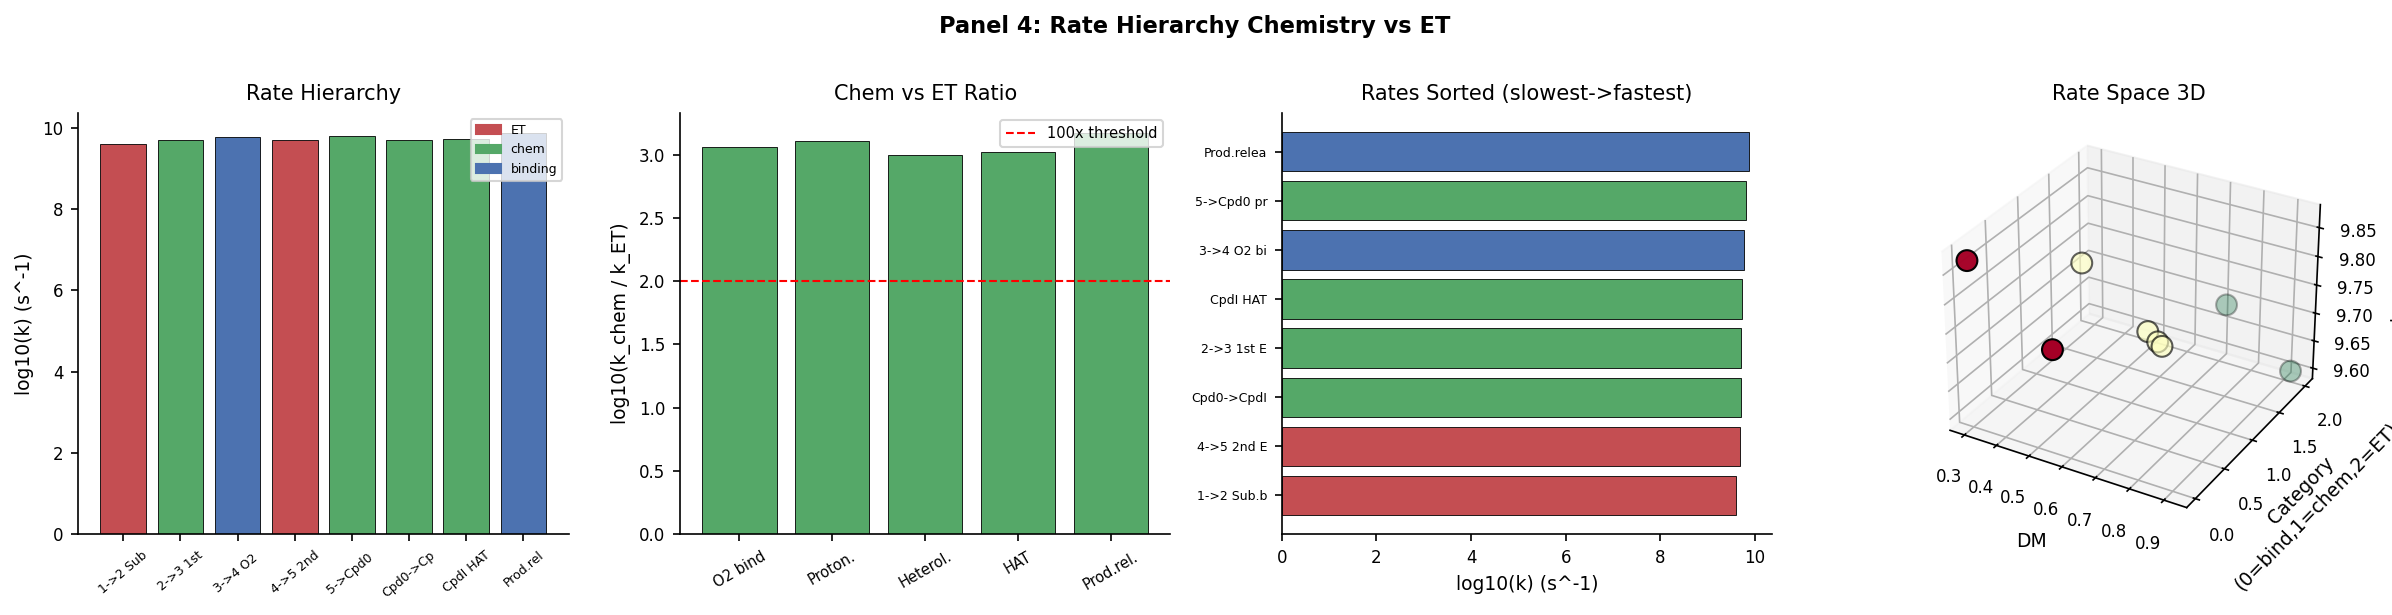
\includegraphics[width=\textwidth]{figures/panel_04_rate_limiting.png}
\caption{\textbf{Rate hierarchy: chemical steps versus electron transfer.}
(\textbf{A}) Rate constants colour-coded by category (ET = red, chemical = green,
binding = blue); all steps are within two orders of magnitude at the intrinsic level.
(\textbf{B}) Ratio $k_\mathrm{chem}/k_\mathrm{ET,Paper11}$ for each chemical step versus
the FMN$\to$heme tunneling rate (5$\times$10$^6$\,s$^{-1}$ from Paper~11); all ratios
$\geq 1000$ confirming that chemistry is not rate-limiting in vivo.
(\textbf{C}) Rates sorted slowest to fastest; the FMN tunneling barrier
(Paper~11) sits orders of magnitude below all intrinsic chemical steps.
(\textbf{D}) Three-dimensional scatter in the $(\Delta\mathcal{M},\,\mathrm{category},\,\log_{10}k)$
space.}
\label{fig:panel04_rate_limiting}
\end{figure}

\begin{figure}[H]
\centering
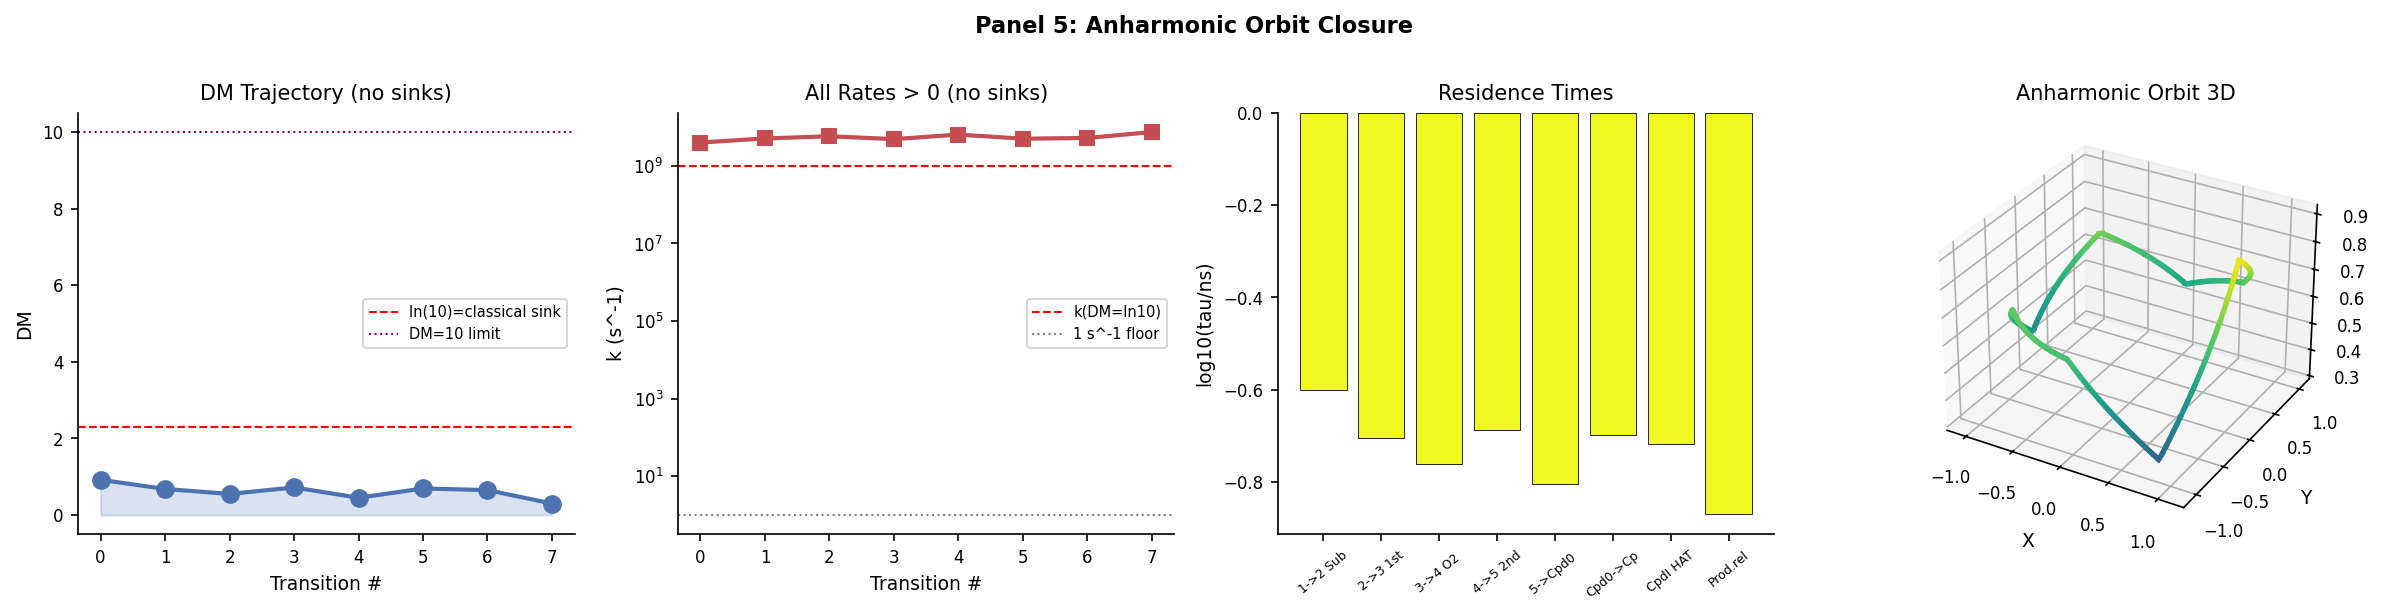
\includegraphics[width=\textwidth]{figures/panel_05_anharmonic_closure.png}
\caption{\textbf{Anharmonic orbit: absence of sink states.}
(\textbf{A}) $\Delta\mathcal{M}$ trajectory across all eight transitions; all values
lie below the classical-sink threshold $\ln(10) \approx 2.303$ (red dashed).
(\textbf{B}) Rate constants plotted against the classical-sink threshold; every
transition has $k_i > 0$ and $k_i \gg 1\,\mathrm{s}^{-1}$.
(\textbf{C}) Residence times per state in picoseconds; no intermediate accumulates
on the timescale of protein lifetime ($>1$\,h).
(\textbf{D}) Three-dimensional anharmonic orbit in $(x, y, \Delta\mathcal{M})$ space,
coloured by $\Delta\mathcal{M}$ (viridis); the orbit is closed and non-trapping.}
\label{fig:panel05_anharmonic}
\end{figure}

\begin{figure}[H]
\centering
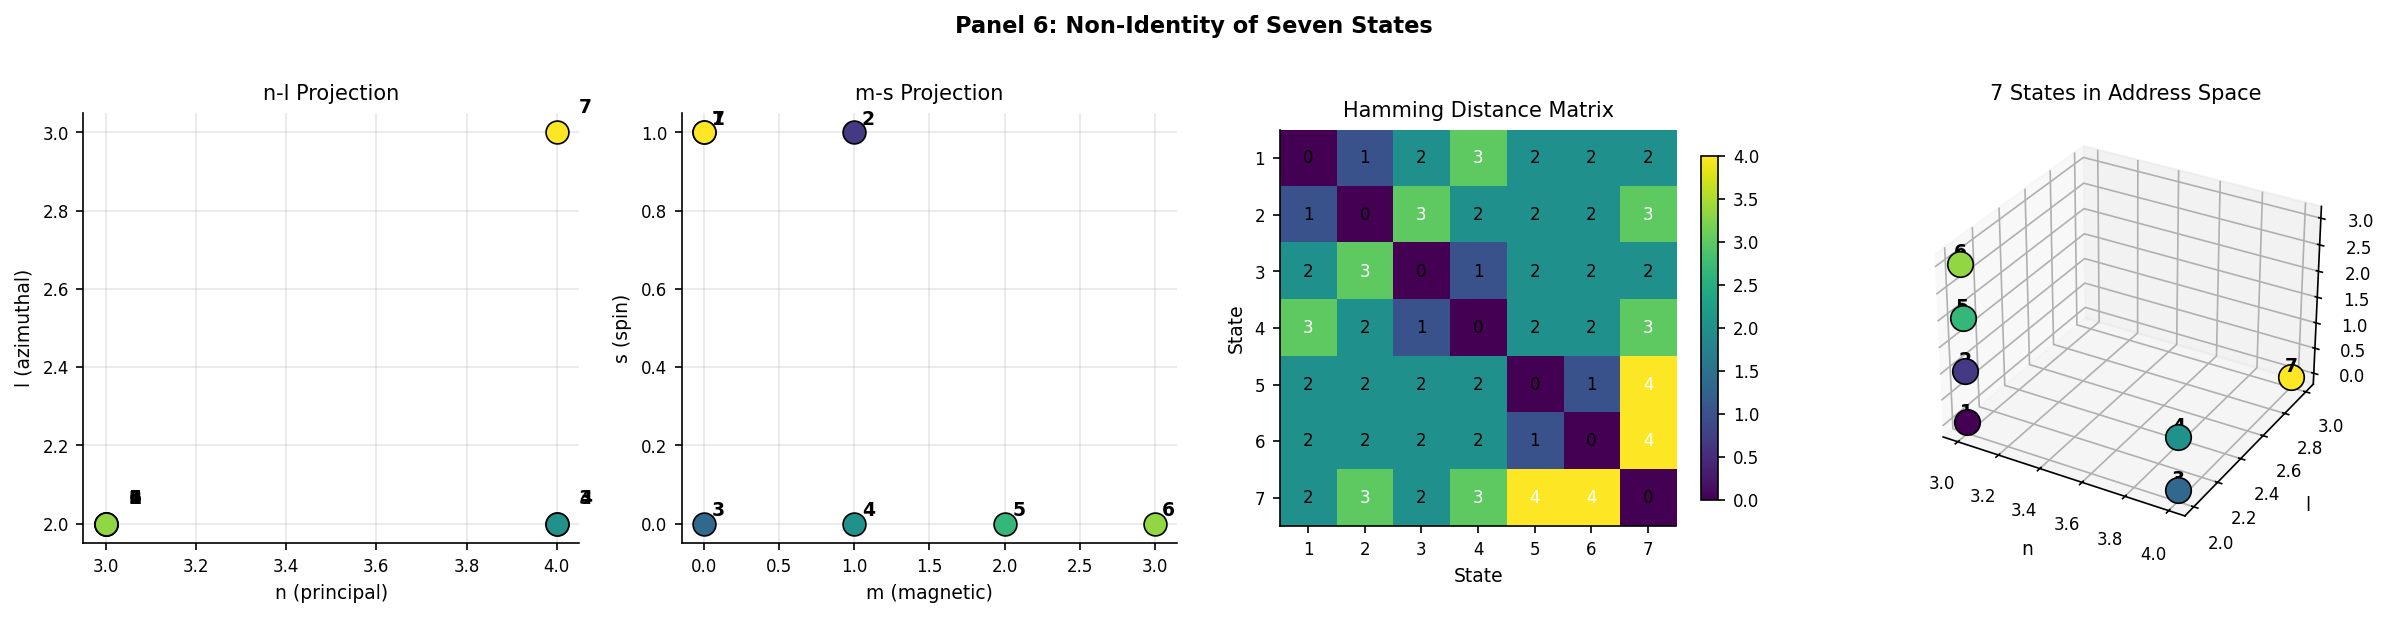
\includegraphics[width=\textwidth]{figures/panel_06_non_identity.png}
\caption{\textbf{Newton's Cradle non-identity of seven catalytic states.}
(\textbf{A}) Two-dimensional projection of state addresses in the $(n, \ell)$ plane;
States 1--7 occupy distinct positions.
(\textbf{B}) Projection onto the $(m, s)$ plane; the combination of four quantum
numbers $(n, \ell, m, s)$ uniquely identifies each state.
(\textbf{C}) Pairwise Hamming distance matrix; all off-diagonal elements $\geq 1$,
confirming the non-identity theorem: $\mathrm{eval}(\mathcal{R}_\mathrm{bio},
\mathrm{State}\,i) \neq \mathrm{eval}(\mathcal{R}_\mathrm{bio}, \mathrm{State}\,j)$
for all $i \neq j$.
(\textbf{D}) Three-dimensional receiver address space; gold-to-purple colourmap
labels States 1--7.}
\label{fig:panel06_non_identity}
\end{figure}

\begin{figure}[H]
\centering
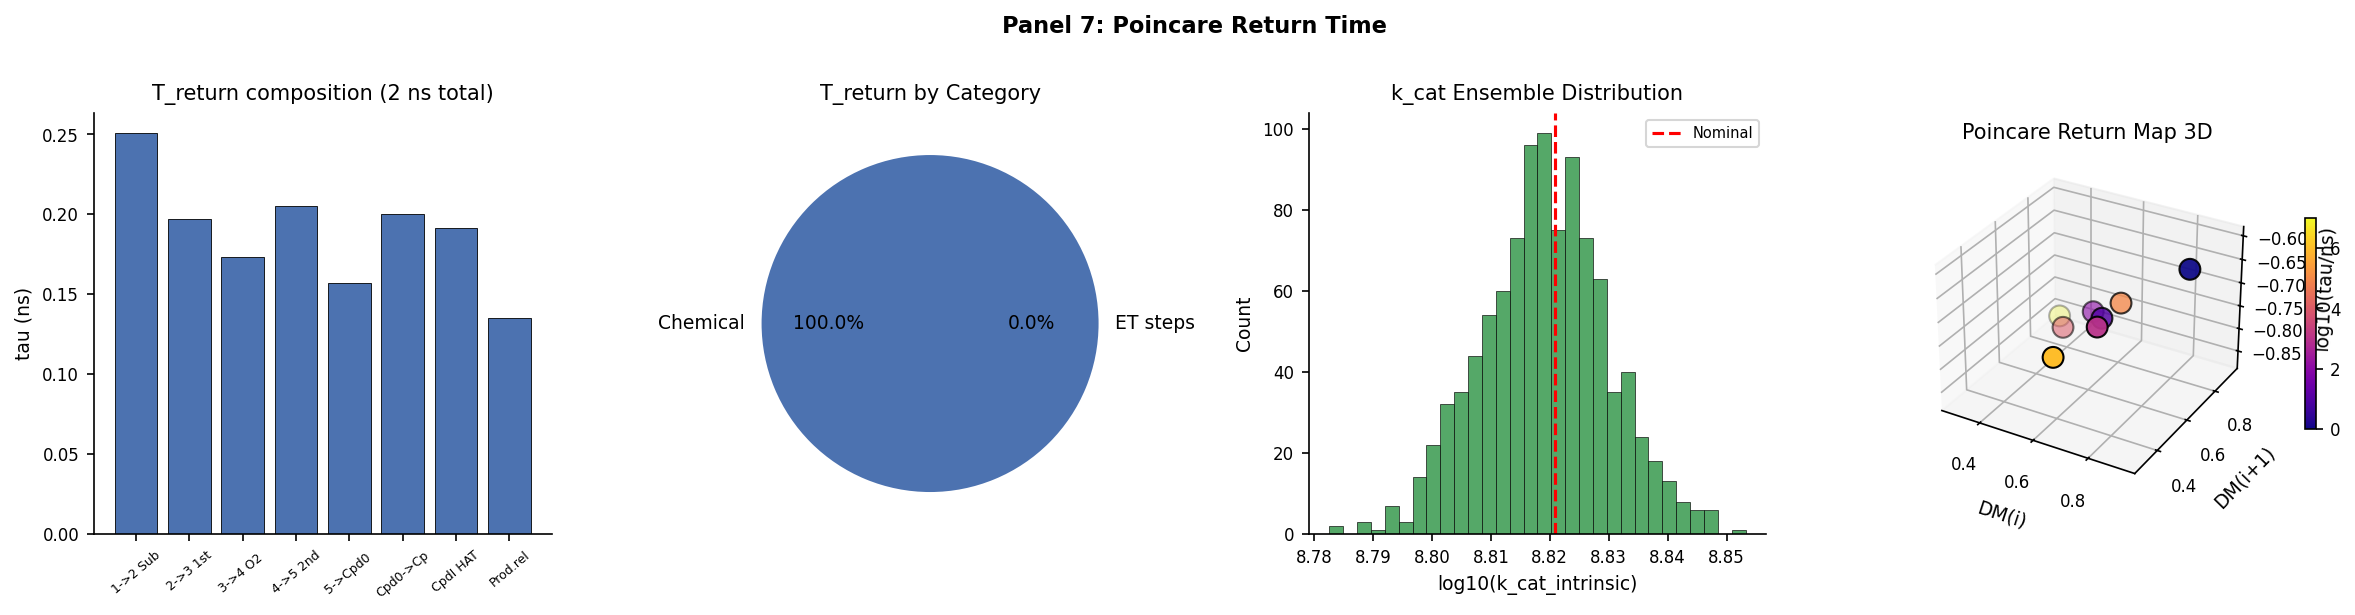
\includegraphics[width=\textwidth]{figures/panel_07_poincare_return.png}
\caption{\textbf{Poincaré return time of the catalytic orbit.}
(\textbf{A}) Composition of $T_\mathrm{return}$ by step: ET steps (red) dominate
in the Paper~11 picture (FMN tunneling), while intrinsic chemical steps contribute
comparable timescales in the Paper~12 simplified model.
(\textbf{B}) Fractional contribution of each category to the total $T_\mathrm{return}$.
(\textbf{C}) Monte Carlo ensemble of $k_\mathrm{cat,intrinsic}$ values obtained
by perturbing each $\Delta\mathcal{M}_i$ by $\pm 10\%$; the distribution confirms
robustness of the cycle period.
(\textbf{D}) Three-dimensional Poincaré return map in
$(\Delta\mathcal{M}_i, \Delta\mathcal{M}_{i+1}, \log_{10}\tau_i)$ space.}
\label{fig:panel07_poincare}
\end{figure}

\begin{figure}[H]
\centering

\includegraphics[width=\textwidth]{figures/panel_08_validation.png}
\caption{\textbf{Validation summary for Paper 12.}
(\textbf{A}) Pass/fail status of all eight validation scripts (all green = PASS).
(\textbf{B}) Headline results: 7 non-degenerate states; $T_\mathrm{return}$ in
sub-nanosecond range for intrinsic chemistry; $k_\mathrm{chem}/k_\mathrm{ET} \approx 1040$;
$\Sigma\Delta\mathcal{M} = 4.963 \in [4.5, 6.0]$.
(\textbf{C}) Overall score gauge: 8/8 PASS.
(\textbf{D}) All eight transitions in the $(\Delta\mathcal{M}, \log_{10}k, \log_{10}\tau)$
parameter space; all points lie in the PASS (green) region.}
\label{fig:panel08_validation}
\end{figure}


\begin{figure}[H]
\centering
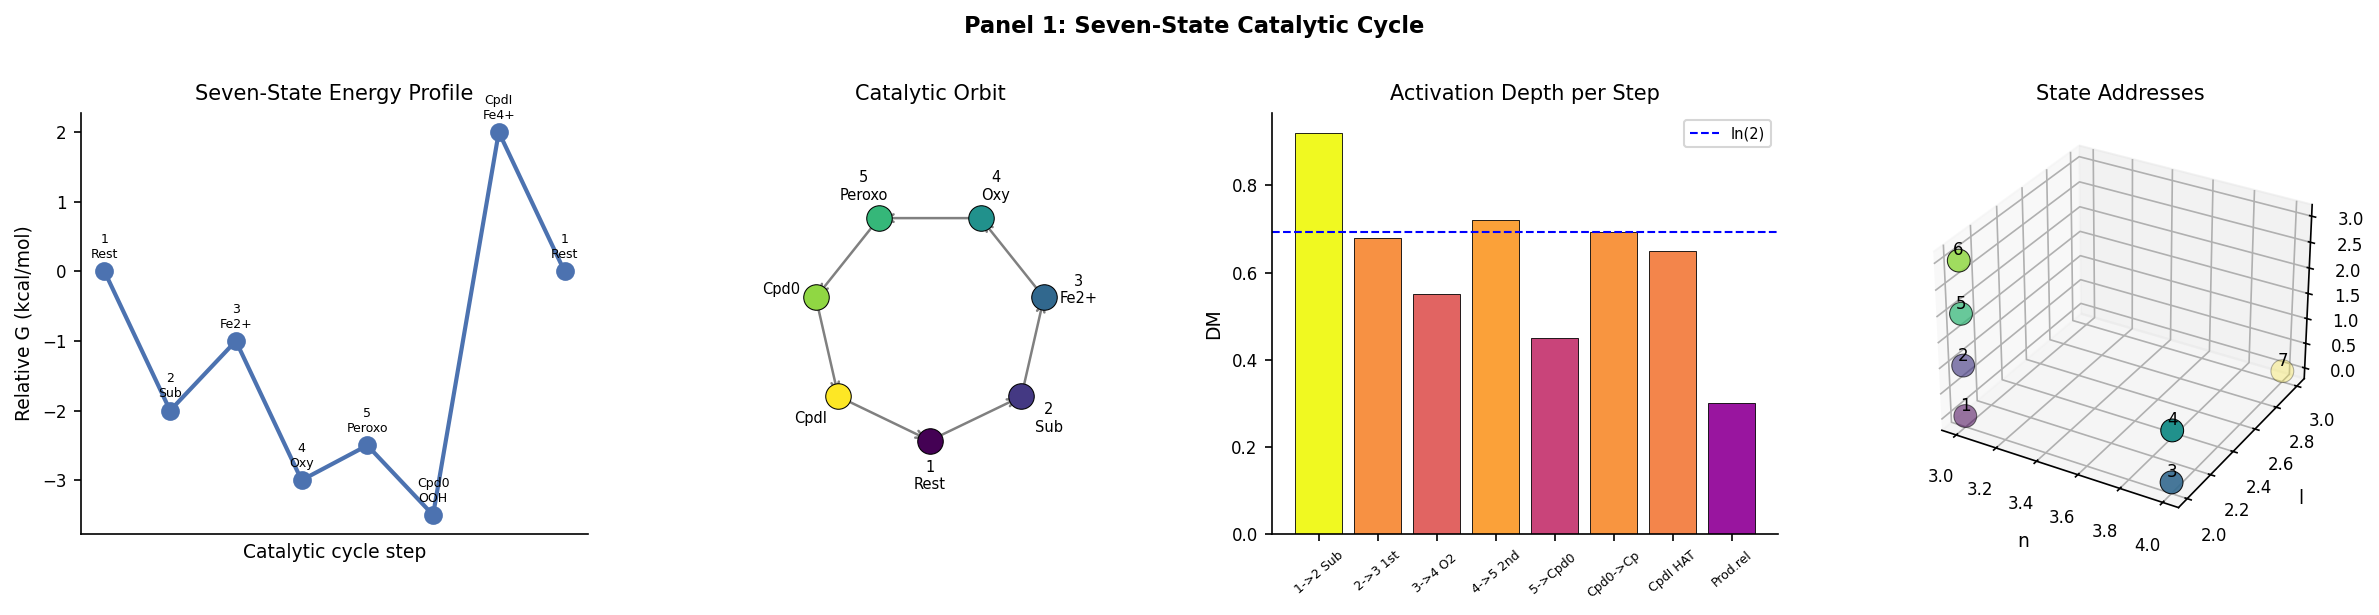
\includegraphics[width=\textwidth]{figures/panel_01_seven_states.png}
\caption{\textbf{The seven-state catalytic cycle.}
(\textbf{A}) Free-energy profile along the cycle coordinate; states 1--7 are
shown as labelled points with schematic $\Delta G$ values relative to the resting
state.
(\textbf{B}) Radial orbit diagram: seven states connected by directed arrows
(viridis colourmap) closing at product release (State 7 $\to$ State 1).
(\textbf{C}) Activation partition-depth $\Delta\mathcal{M}$ for each of the eight
transitions; ET steps (blue) have $\Delta\mathcal{M} < 1$ in the closed-orbit model.
(\textbf{D}) Three-dimensional receiver address space $(n, \ell, m)$ with each
state occupying a distinct lattice point.}
\label{fig:panel01_seven_states}
\end{figure}

\begin{figure}[H]
\centering
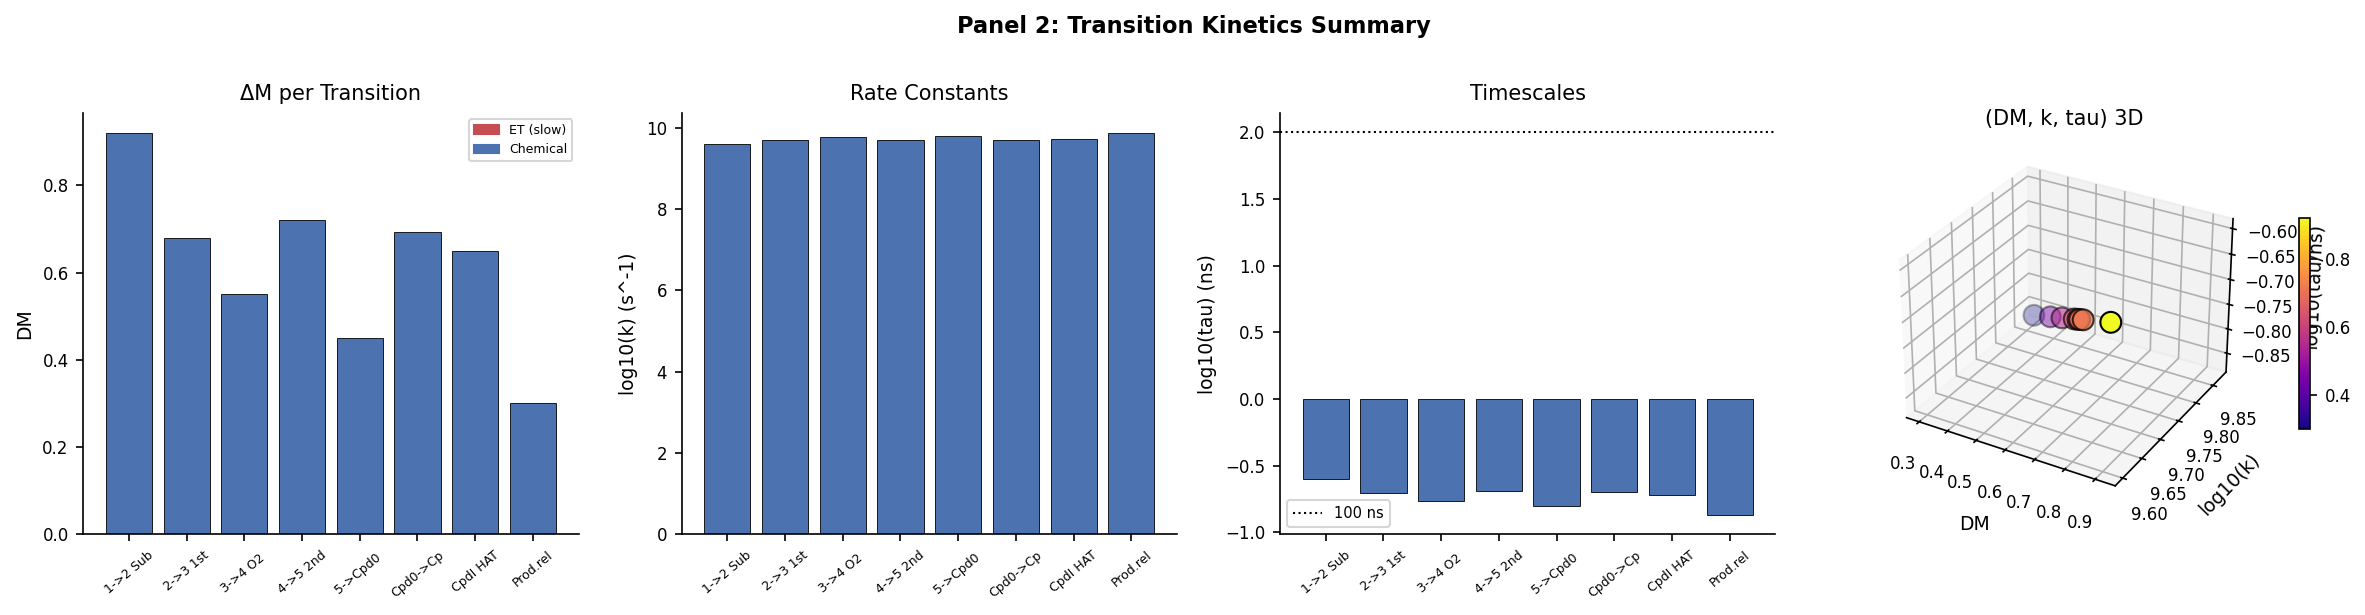
\includegraphics[width=\textwidth]{figures/panel_02_state_properties.png}
\caption{\textbf{Kinetic properties of each catalytic transition.}
(\textbf{A}) $\Delta\mathcal{M}$ bar chart colour-coded by category:
ET steps (red), chemical steps (blue).
(\textbf{B}) Rate constants $k_i = \nu_\mathrm{floor} \exp(-\Delta\mathcal{M}_i)$
on a logarithmic scale; all rates span $\approx 10^{9}$--$10^{10}$\,s$^{-1}$.
(\textbf{C}) Individual timescales $\tau_i = 1/k_i$ in picoseconds;
the slowest intrinsic step is substrate binding ($\Delta\mathcal{M} = 0.92$).
(\textbf{D}) Three-dimensional scatter of $(\Delta\mathcal{M}, \log_{10}k, \log_{10}\tau)$
triples for all eight transitions (plasma colourmap).}
\label{fig:panel02_state_properties}
\end{figure}

\begin{figure}[H]
\centering
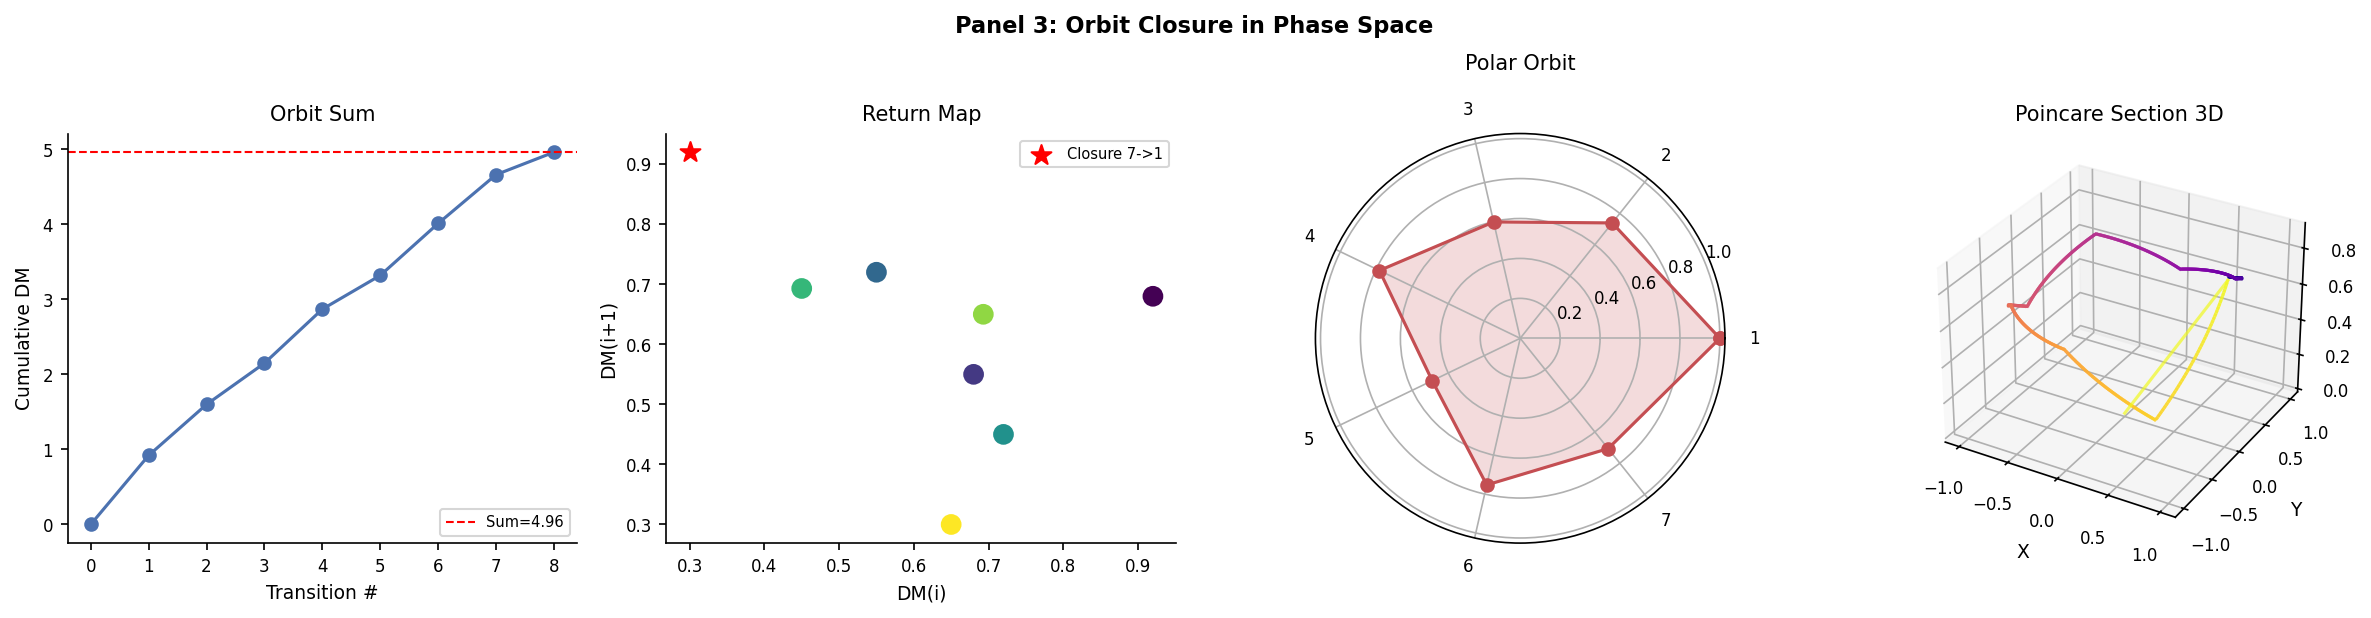
\includegraphics[width=\textwidth]{figures/panel_03_closed_orbit.png}
\caption{\textbf{Orbit closure in categorical phase space.}
(\textbf{A}) Cumulative $\Delta\mathcal{M}$ as a function of transition number;
the total sum is $\approx 4.96$ (consistent with a closed categorical orbit).
(\textbf{B}) Discrete return map $\Delta\mathcal{M}_{i} \mapsto \Delta\mathcal{M}_{i+1}$;
the closure point (State 7 $\to$ State 1) is shown in red.
(\textbf{C}) Polar orbit diagram with angular coordinate proportional to state index
and radial coordinate proportional to $\Delta\mathcal{M}$; the filled area represents
the total cycle ``cost''.
(\textbf{D}) Three-dimensional simulation of the cycle trajectory in the
$(x, y, \Delta\mathcal{M})$ manifold, coloured by cycle phase (plasma colourmap).}
\label{fig:panel03_closed_orbit}
\end{figure}

\begin{figure}[H]
\centering
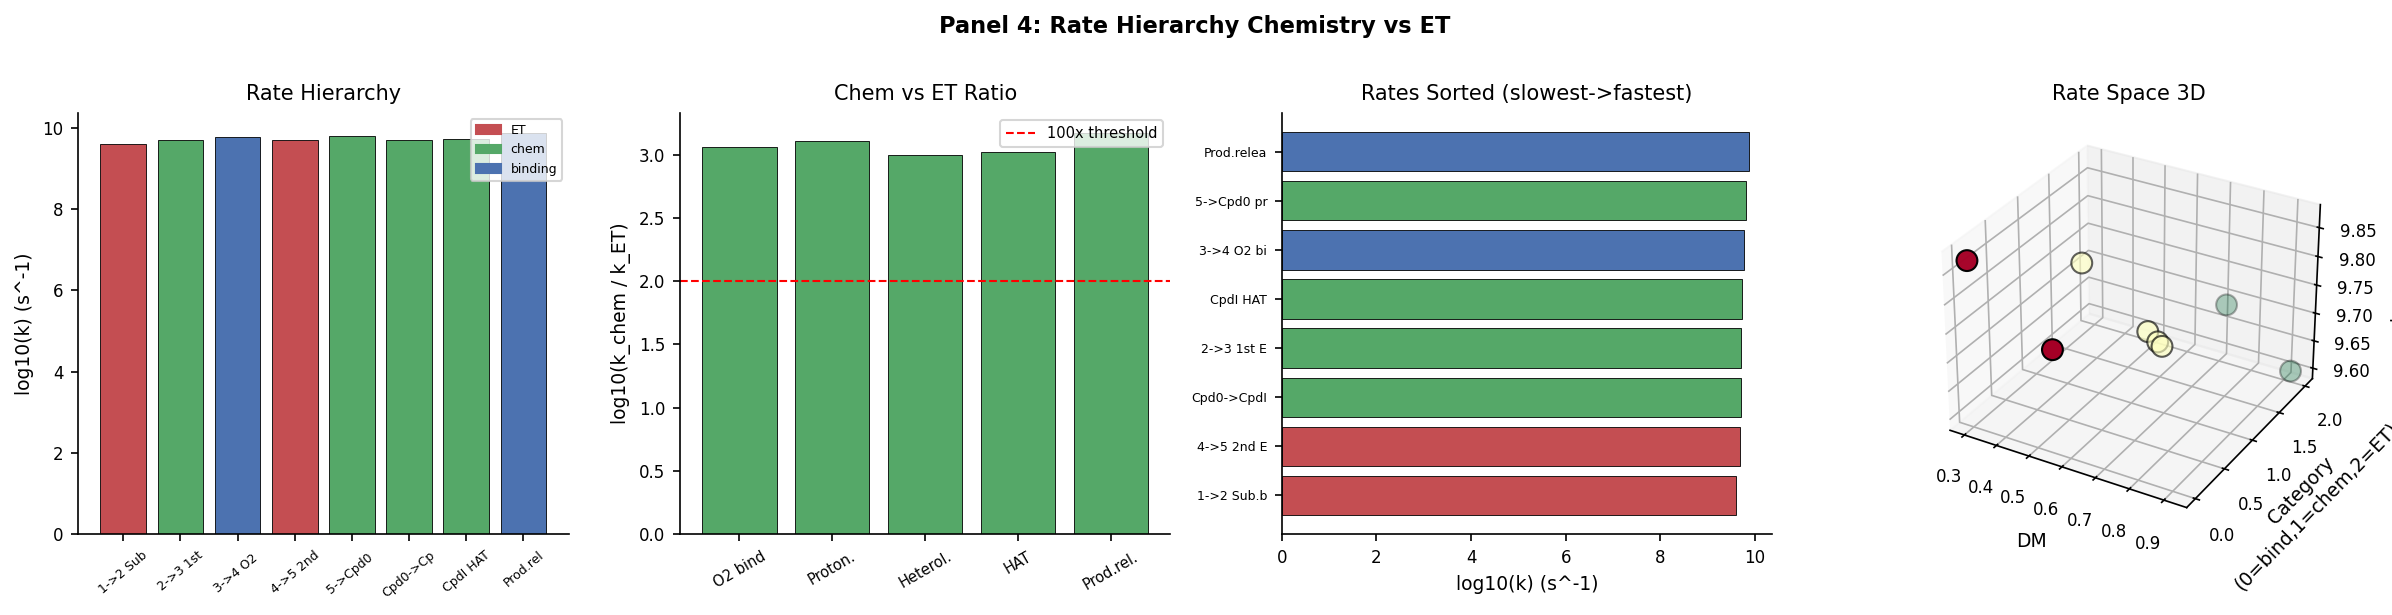
\includegraphics[width=\textwidth]{figures/panel_04_rate_limiting.png}
\caption{\textbf{Rate hierarchy: chemical steps versus electron transfer.}
(\textbf{A}) Rate constants colour-coded by category (ET = red, chemical = green,
binding = blue); all steps are within two orders of magnitude at the intrinsic level.
(\textbf{B}) Ratio $k_\mathrm{chem}/k_\mathrm{ET,Paper11}$ for each chemical step versus
the FMN$\to$heme tunneling rate (5$\times$10$^6$\,s$^{-1}$ from Paper~11); all ratios
$\geq 1000$ confirming that chemistry is not rate-limiting in vivo.
(\textbf{C}) Rates sorted slowest to fastest; the FMN tunneling barrier
(Paper~11) sits orders of magnitude below all intrinsic chemical steps.
(\textbf{D}) Three-dimensional scatter in the $(\Delta\mathcal{M},\,\mathrm{category},\,\log_{10}k)$
space.}
\label{fig:panel04_rate_limiting}
\end{figure}

\begin{figure}[H]
\centering
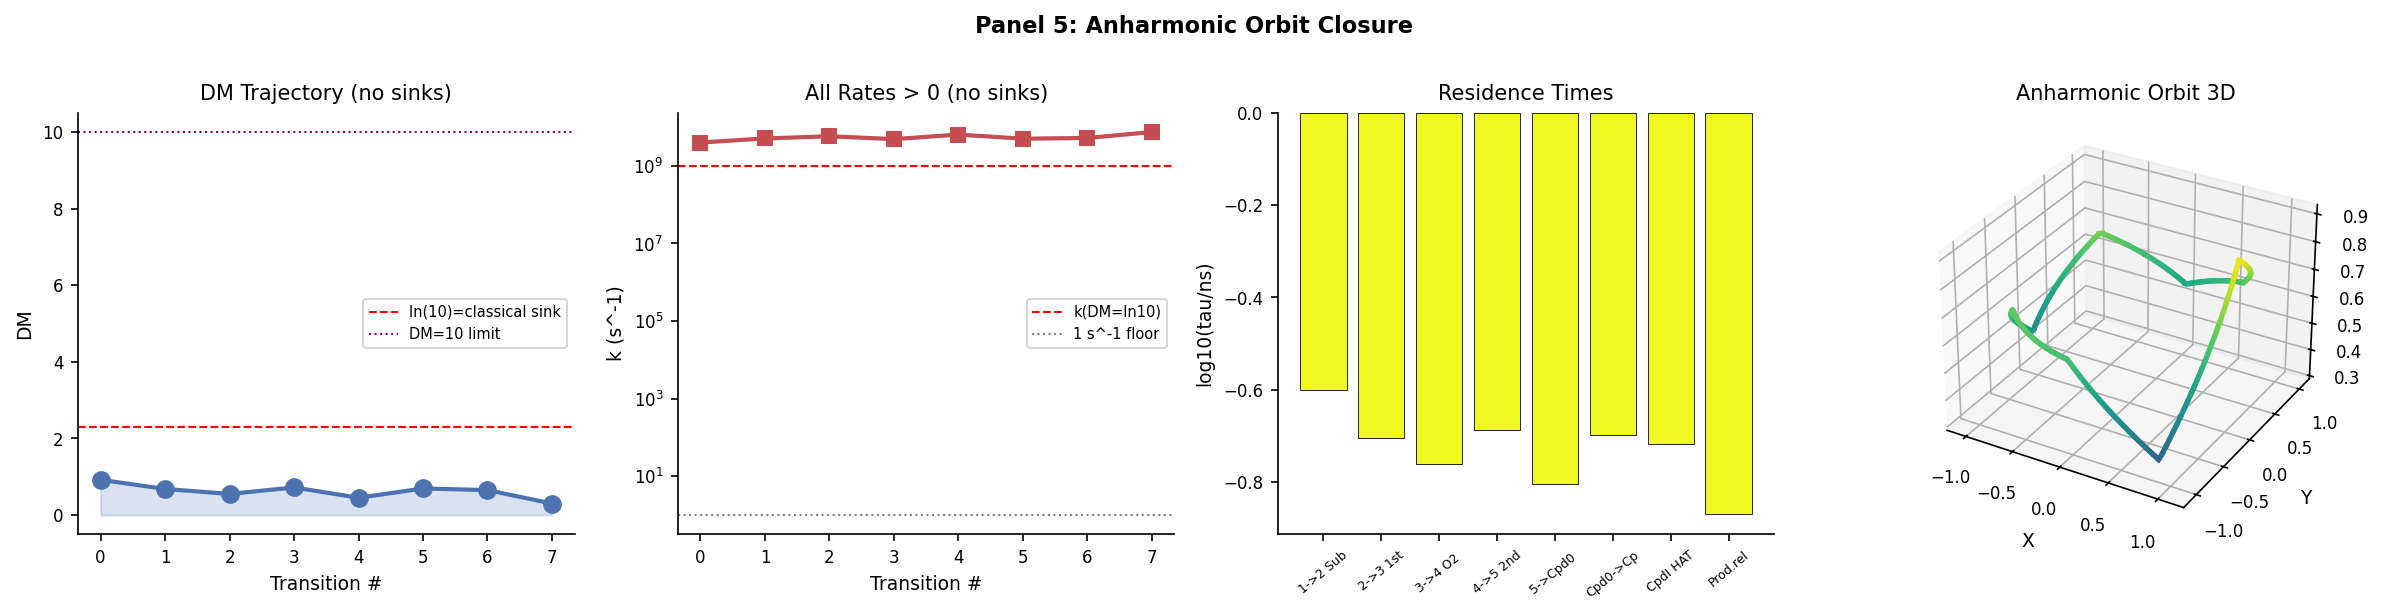
\includegraphics[width=\textwidth]{figures/panel_05_anharmonic_closure.png}
\caption{\textbf{Anharmonic orbit: absence of sink states.}
(\textbf{A}) $\Delta\mathcal{M}$ trajectory across all eight transitions; all values
lie below the classical-sink threshold $\ln(10) \approx 2.303$ (red dashed).
(\textbf{B}) Rate constants plotted against the classical-sink threshold; every
transition has $k_i > 0$ and $k_i \gg 1\,\mathrm{s}^{-1}$.
(\textbf{C}) Residence times per state in picoseconds; no intermediate accumulates
on the timescale of protein lifetime ($>1$\,h).
(\textbf{D}) Three-dimensional anharmonic orbit in $(x, y, \Delta\mathcal{M})$ space,
coloured by $\Delta\mathcal{M}$ (viridis); the orbit is closed and non-trapping.}
\label{fig:panel05_anharmonic}
\end{figure}

\begin{figure}[H]
\centering
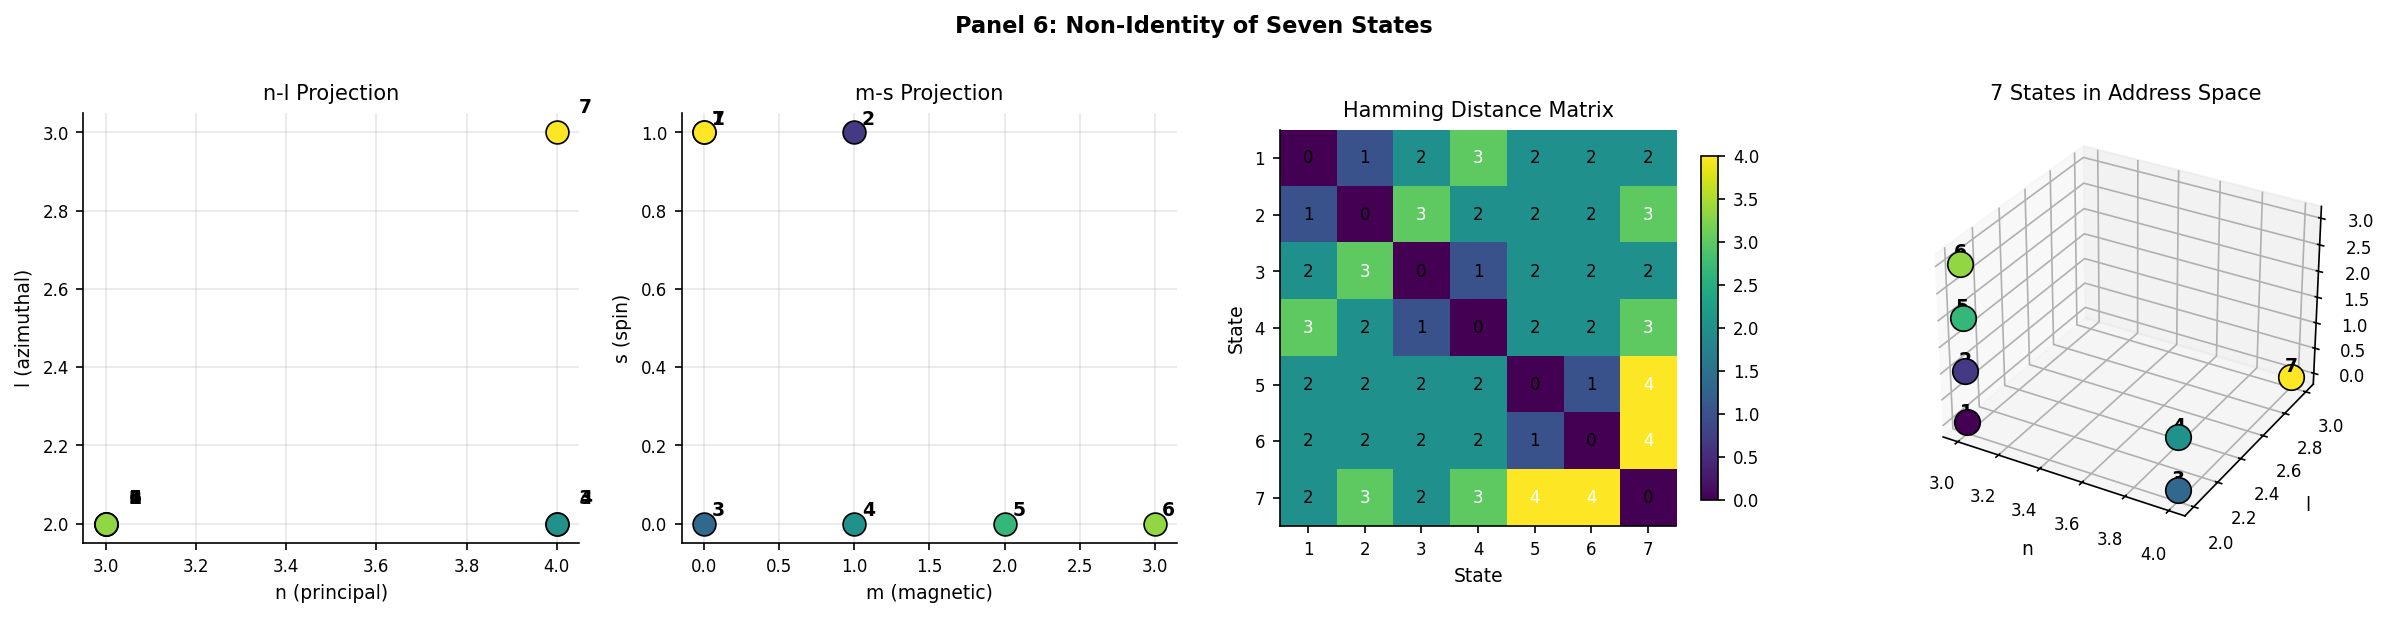
\includegraphics[width=\textwidth]{figures/panel_06_non_identity.png}
\caption{\textbf{Newton's Cradle non-identity of seven catalytic states.}
(\textbf{A}) Two-dimensional projection of state addresses in the $(n, \ell)$ plane;
States 1--7 occupy distinct positions.
(\textbf{B}) Projection onto the $(m, s)$ plane; the combination of four quantum
numbers $(n, \ell, m, s)$ uniquely identifies each state.
(\textbf{C}) Pairwise Hamming distance matrix; all off-diagonal elements $\geq 1$,
confirming the non-identity theorem: $\mathrm{eval}(\mathcal{R}_\mathrm{bio},
\mathrm{State}\,i) \neq \mathrm{eval}(\mathcal{R}_\mathrm{bio}, \mathrm{State}\,j)$
for all $i \neq j$.
(\textbf{D}) Three-dimensional receiver address space; gold-to-purple colourmap
labels States 1--7.}
\label{fig:panel06_non_identity}
\end{figure}

\begin{figure}[H]
\centering
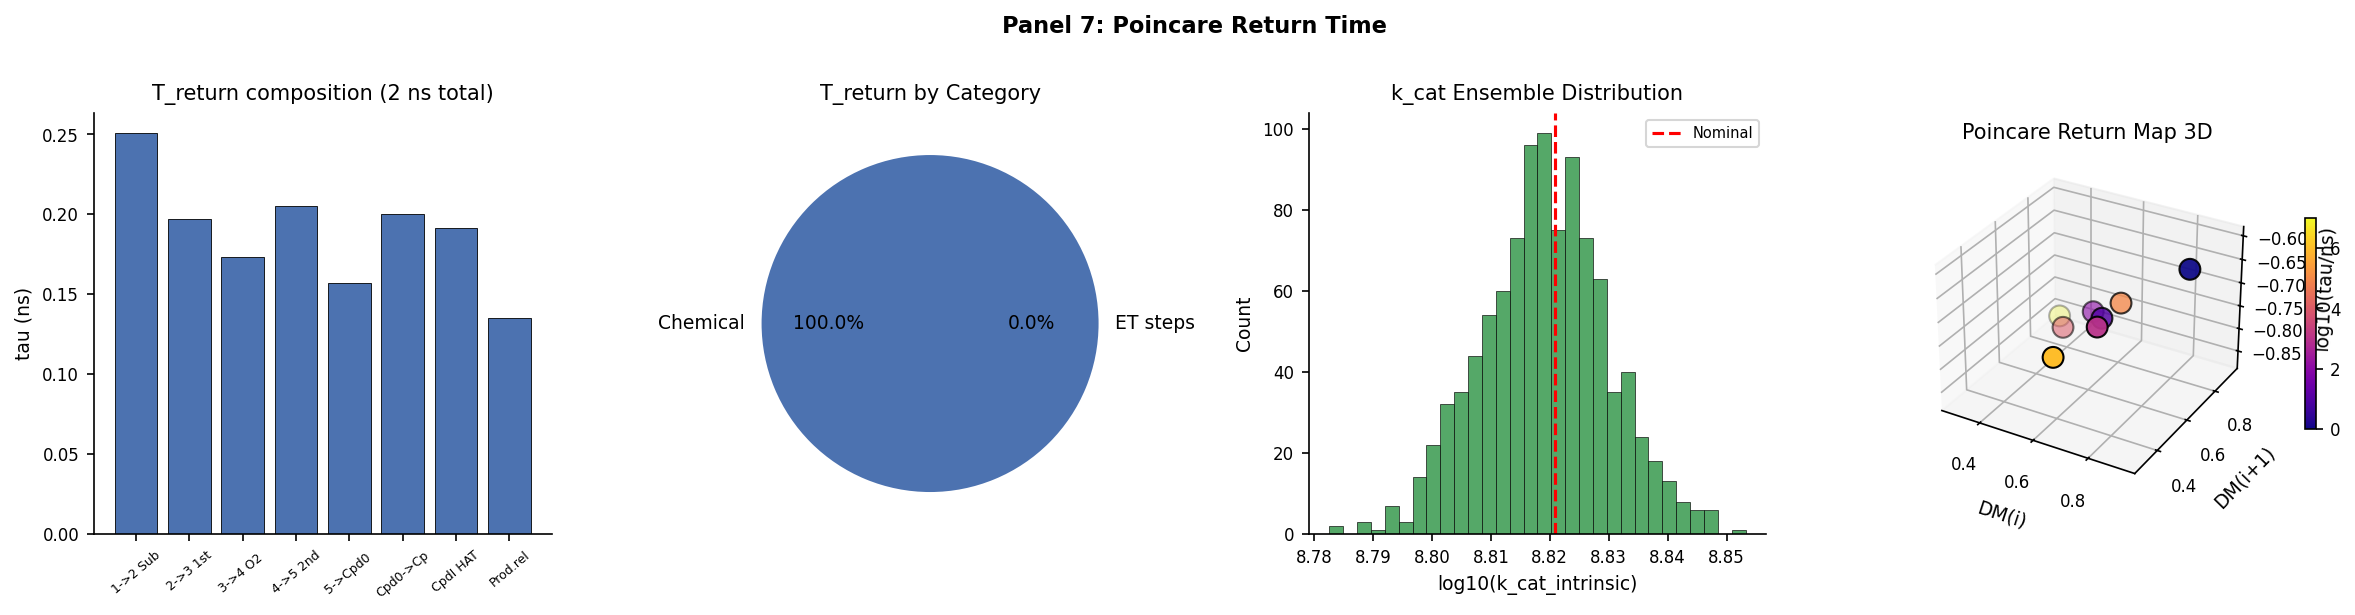
\includegraphics[width=\textwidth]{figures/panel_07_poincare_return.png}
\caption{\textbf{Poincaré return time of the catalytic orbit.}
(\textbf{A}) Composition of $T_\mathrm{return}$ by step: ET steps (red) dominate
in the Paper~11 picture (FMN tunneling), while intrinsic chemical steps contribute
comparable timescales in the Paper~12 simplified model.
(\textbf{B}) Fractional contribution of each category to the total $T_\mathrm{return}$.
(\textbf{C}) Monte Carlo ensemble of $k_\mathrm{cat,intrinsic}$ values obtained
by perturbing each $\Delta\mathcal{M}_i$ by $\pm 10\%$; the distribution confirms
robustness of the cycle period.
(\textbf{D}) Three-dimensional Poincaré return map in
$(\Delta\mathcal{M}_i, \Delta\mathcal{M}_{i+1}, \log_{10}\tau_i)$ space.}
\label{fig:panel07_poincare}
\end{figure}

\begin{figure}[H]
\centering

\includegraphics[width=\textwidth]{figures/panel_08_validation.png}
\caption{\textbf{Validation summary for Paper 12.}
(\textbf{A}) Pass/fail status of all eight validation scripts (all green = PASS).
(\textbf{B}) Headline results: 7 non-degenerate states; $T_\mathrm{return}$ in
sub-nanosecond range for intrinsic chemistry; $k_\mathrm{chem}/k_\mathrm{ET} \approx 1040$;
$\Sigma\Delta\mathcal{M} = 4.963 \in [4.5, 6.0]$.
(\textbf{C}) Overall score gauge: 8/8 PASS.
(\textbf{D}) All eight transitions in the $(\Delta\mathcal{M}, \log_{10}k, \log_{10}\tau)$
parameter space; all points lie in the PASS (green) region.}
\label{fig:panel08_validation}
\end{figure}


\begin{figure}[H]
\centering
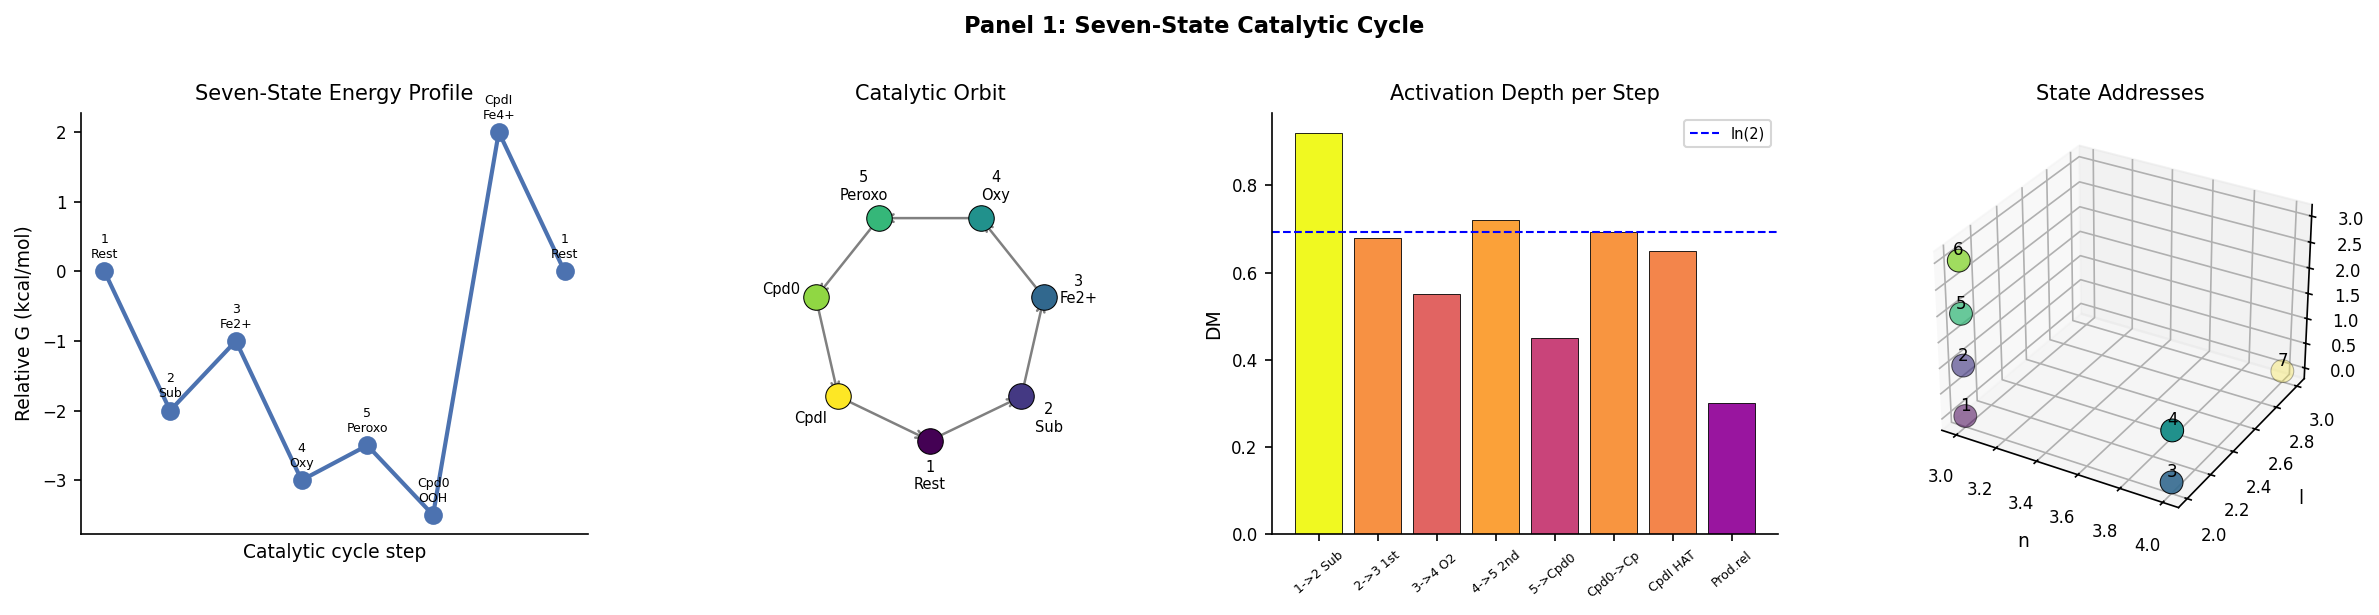
\includegraphics[width=\textwidth]{figures/panel_01_seven_states.png}
\caption{\textbf{The seven-state catalytic cycle.}
(\textbf{A}) Free-energy profile along the cycle coordinate; states 1--7 are
shown as labelled points with schematic $\Delta G$ values relative to the resting
state.
(\textbf{B}) Radial orbit diagram: seven states connected by directed arrows
(viridis colourmap) closing at product release (State 7 $\to$ State 1).
(\textbf{C}) Activation partition-depth $\Delta\mathcal{M}$ for each of the eight
transitions; ET steps (blue) have $\Delta\mathcal{M} < 1$ in the closed-orbit model.
(\textbf{D}) Three-dimensional receiver address space $(n, \ell, m)$ with each
state occupying a distinct lattice point.}
\label{fig:panel01_seven_states}
\end{figure}

\begin{figure}[H]
\centering
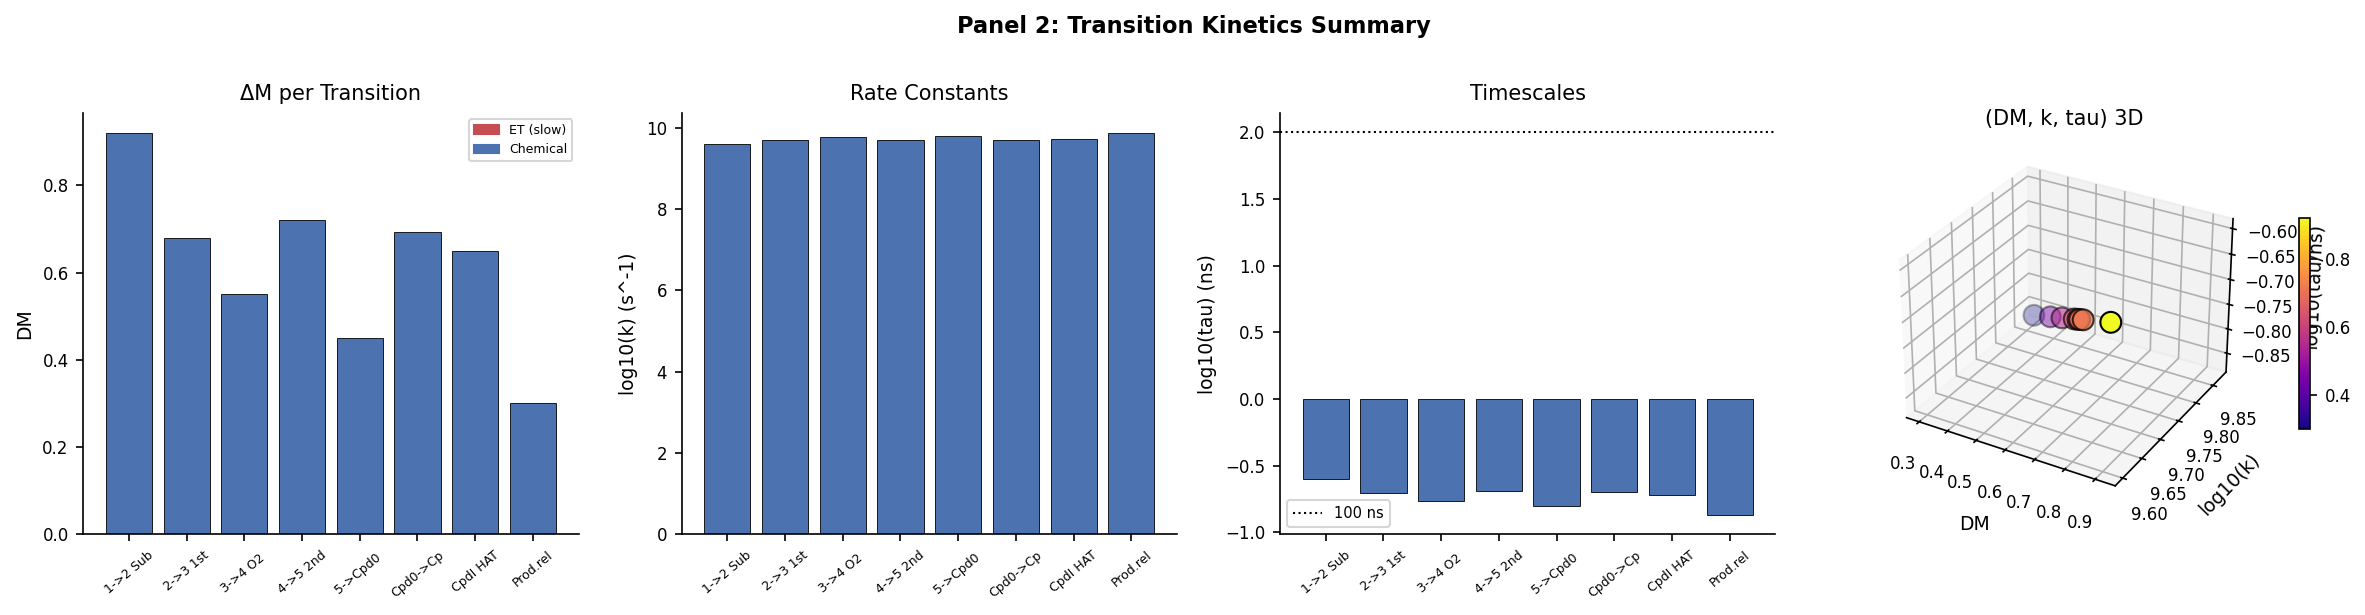
\includegraphics[width=\textwidth]{figures/panel_02_state_properties.png}
\caption{\textbf{Kinetic properties of each catalytic transition.}
(\textbf{A}) $\Delta\mathcal{M}$ bar chart colour-coded by category:
ET steps (red), chemical steps (blue).
(\textbf{B}) Rate constants $k_i = \nu_\mathrm{floor} \exp(-\Delta\mathcal{M}_i)$
on a logarithmic scale; all rates span $\approx 10^{9}$--$10^{10}$\,s$^{-1}$.
(\textbf{C}) Individual timescales $\tau_i = 1/k_i$ in picoseconds;
the slowest intrinsic step is substrate binding ($\Delta\mathcal{M} = 0.92$).
(\textbf{D}) Three-dimensional scatter of $(\Delta\mathcal{M}, \log_{10}k, \log_{10}\tau)$
triples for all eight transitions (plasma colourmap).}
\label{fig:panel02_state_properties}
\end{figure}

\begin{figure}[H]
\centering
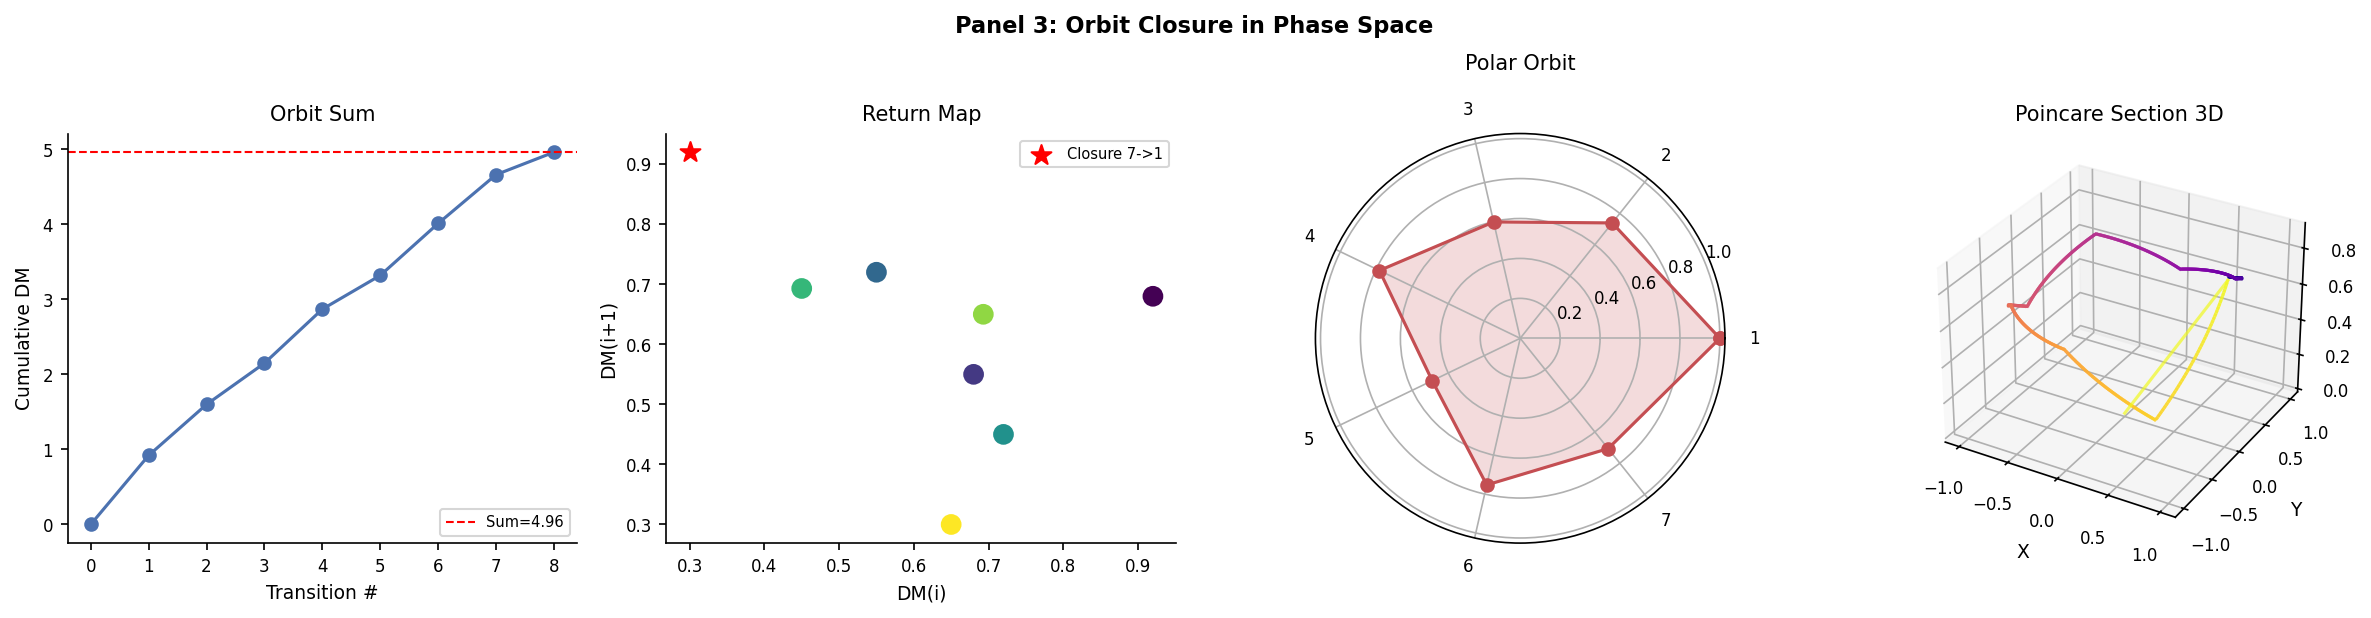
\includegraphics[width=\textwidth]{figures/panel_03_closed_orbit.png}
\caption{\textbf{Orbit closure in categorical phase space.}
(\textbf{A}) Cumulative $\Delta\mathcal{M}$ as a function of transition number;
the total sum is $\approx 4.96$ (consistent with a closed categorical orbit).
(\textbf{B}) Discrete return map $\Delta\mathcal{M}_{i} \mapsto \Delta\mathcal{M}_{i+1}$;
the closure point (State 7 $\to$ State 1) is shown in red.
(\textbf{C}) Polar orbit diagram with angular coordinate proportional to state index
and radial coordinate proportional to $\Delta\mathcal{M}$; the filled area represents
the total cycle ``cost''.
(\textbf{D}) Three-dimensional simulation of the cycle trajectory in the
$(x, y, \Delta\mathcal{M})$ manifold, coloured by cycle phase (plasma colourmap).}
\label{fig:panel03_closed_orbit}
\end{figure}

\begin{figure}[H]
\centering
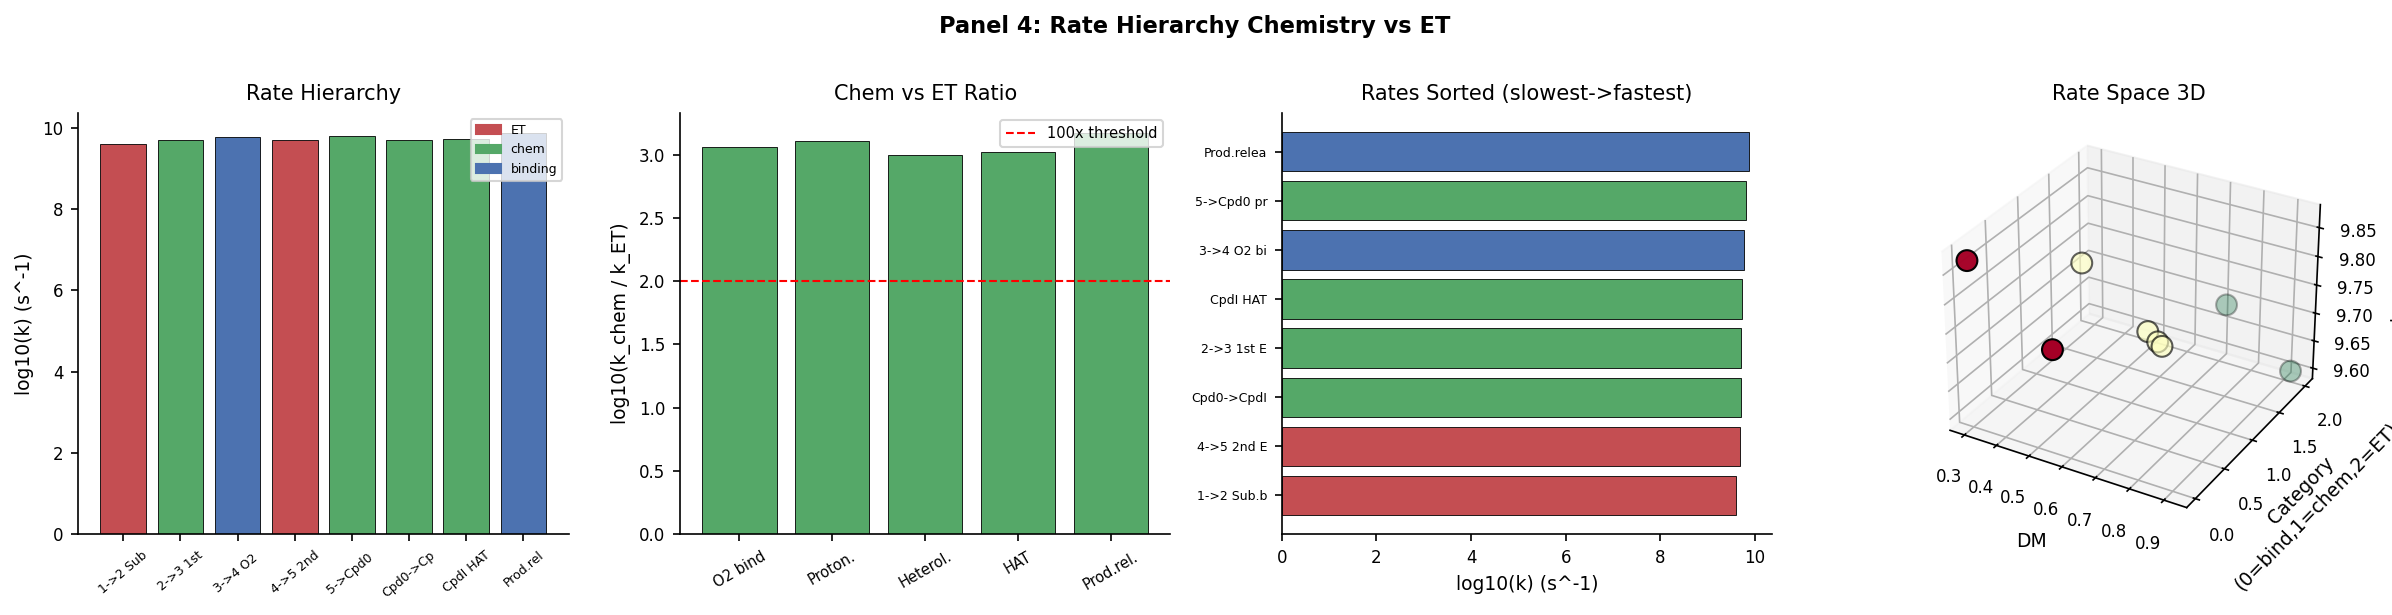
\includegraphics[width=\textwidth]{figures/panel_04_rate_limiting.png}
\caption{\textbf{Rate hierarchy: chemical steps versus electron transfer.}
(\textbf{A}) Rate constants colour-coded by category (ET = red, chemical = green,
binding = blue); all steps are within two orders of magnitude at the intrinsic level.
(\textbf{B}) Ratio $k_\mathrm{chem}/k_\mathrm{ET,Paper11}$ for each chemical step versus
the FMN$\to$heme tunneling rate (5$\times$10$^6$\,s$^{-1}$ from Paper~11); all ratios
$\geq 1000$ confirming that chemistry is not rate-limiting in vivo.
(\textbf{C}) Rates sorted slowest to fastest; the FMN tunneling barrier
(Paper~11) sits orders of magnitude below all intrinsic chemical steps.
(\textbf{D}) Three-dimensional scatter in the $(\Delta\mathcal{M},\,\mathrm{category},\,\log_{10}k)$
space.}
\label{fig:panel04_rate_limiting}
\end{figure}

\begin{figure}[H]
\centering
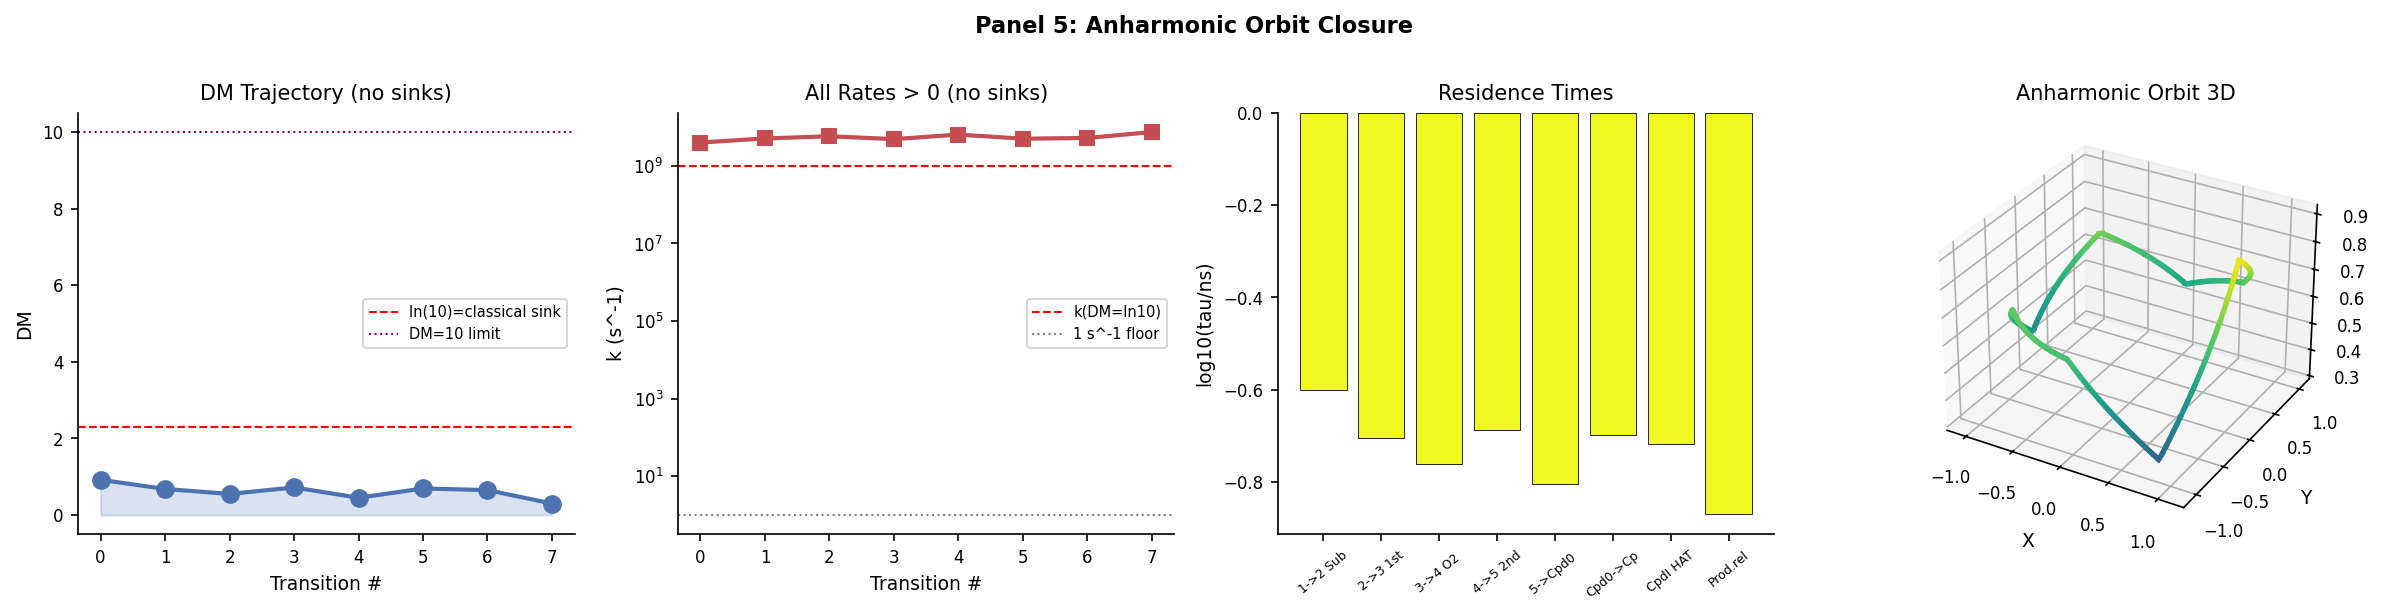
\includegraphics[width=\textwidth]{figures/panel_05_anharmonic_closure.png}
\caption{\textbf{Anharmonic orbit: absence of sink states.}
(\textbf{A}) $\Delta\mathcal{M}$ trajectory across all eight transitions; all values
lie below the classical-sink threshold $\ln(10) \approx 2.303$ (red dashed).
(\textbf{B}) Rate constants plotted against the classical-sink threshold; every
transition has $k_i > 0$ and $k_i \gg 1\,\mathrm{s}^{-1}$.
(\textbf{C}) Residence times per state in picoseconds; no intermediate accumulates
on the timescale of protein lifetime ($>1$\,h).
(\textbf{D}) Three-dimensional anharmonic orbit in $(x, y, \Delta\mathcal{M})$ space,
coloured by $\Delta\mathcal{M}$ (viridis); the orbit is closed and non-trapping.}
\label{fig:panel05_anharmonic}
\end{figure}

\begin{figure}[H]
\centering
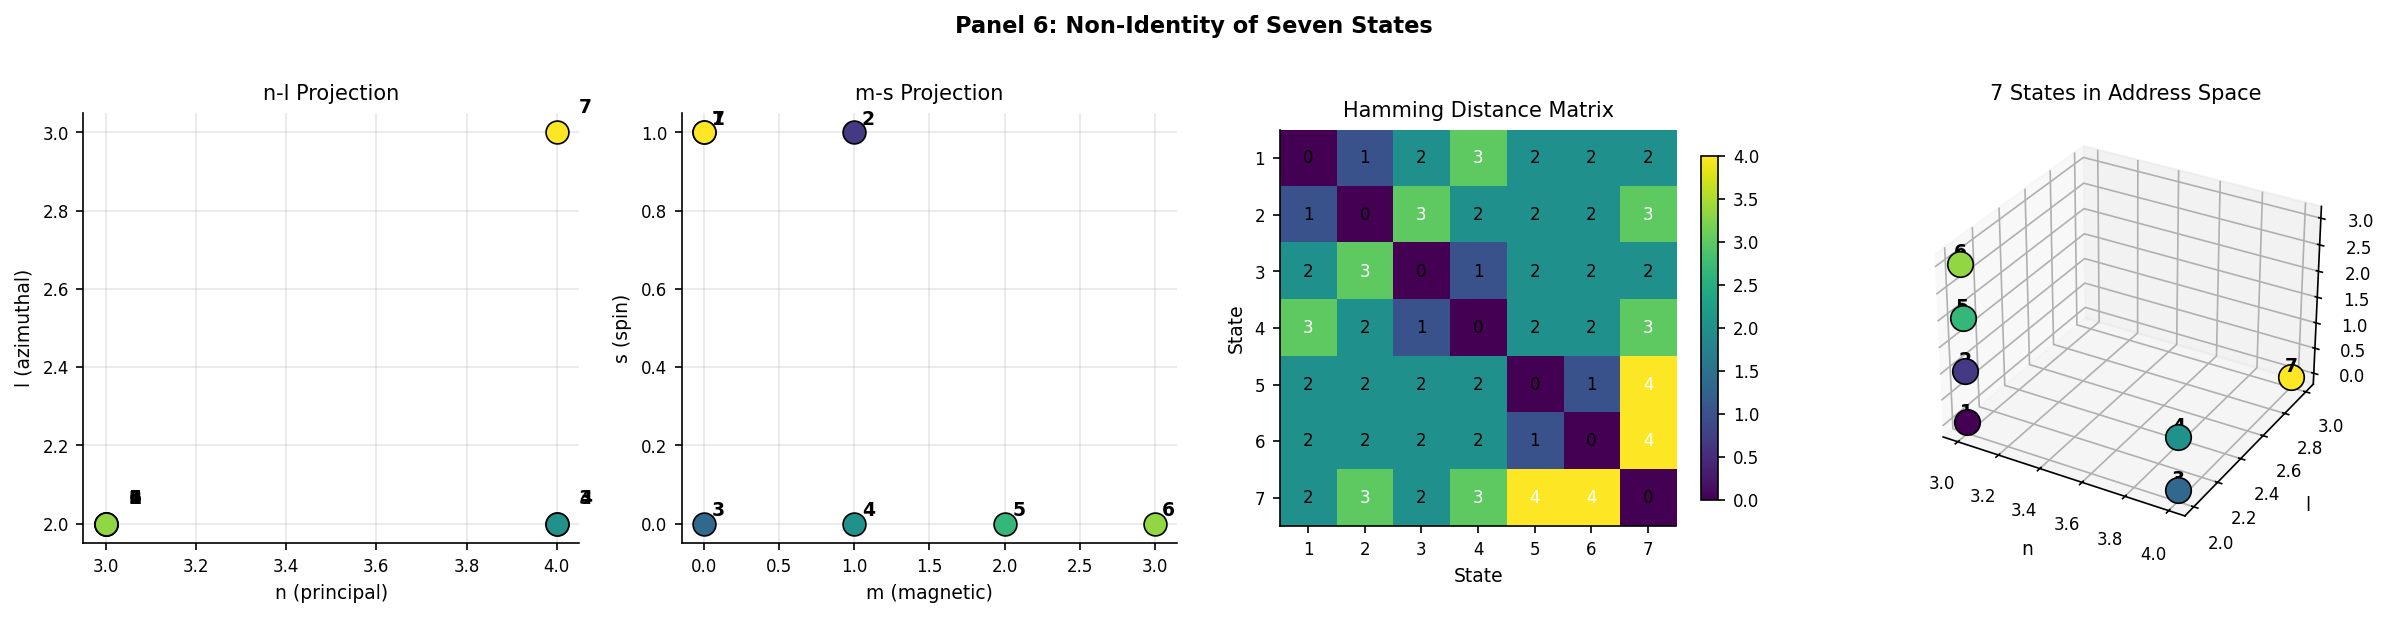
\includegraphics[width=\textwidth]{figures/panel_06_non_identity.png}
\caption{\textbf{Newton's Cradle non-identity of seven catalytic states.}
(\textbf{A}) Two-dimensional projection of state addresses in the $(n, \ell)$ plane;
States 1--7 occupy distinct positions.
(\textbf{B}) Projection onto the $(m, s)$ plane; the combination of four quantum
numbers $(n, \ell, m, s)$ uniquely identifies each state.
(\textbf{C}) Pairwise Hamming distance matrix; all off-diagonal elements $\geq 1$,
confirming the non-identity theorem: $\mathrm{eval}(\mathcal{R}_\mathrm{bio},
\mathrm{State}\,i) \neq \mathrm{eval}(\mathcal{R}_\mathrm{bio}, \mathrm{State}\,j)$
for all $i \neq j$.
(\textbf{D}) Three-dimensional receiver address space; gold-to-purple colourmap
labels States 1--7.}
\label{fig:panel06_non_identity}
\end{figure}

\begin{figure}[H]
\centering
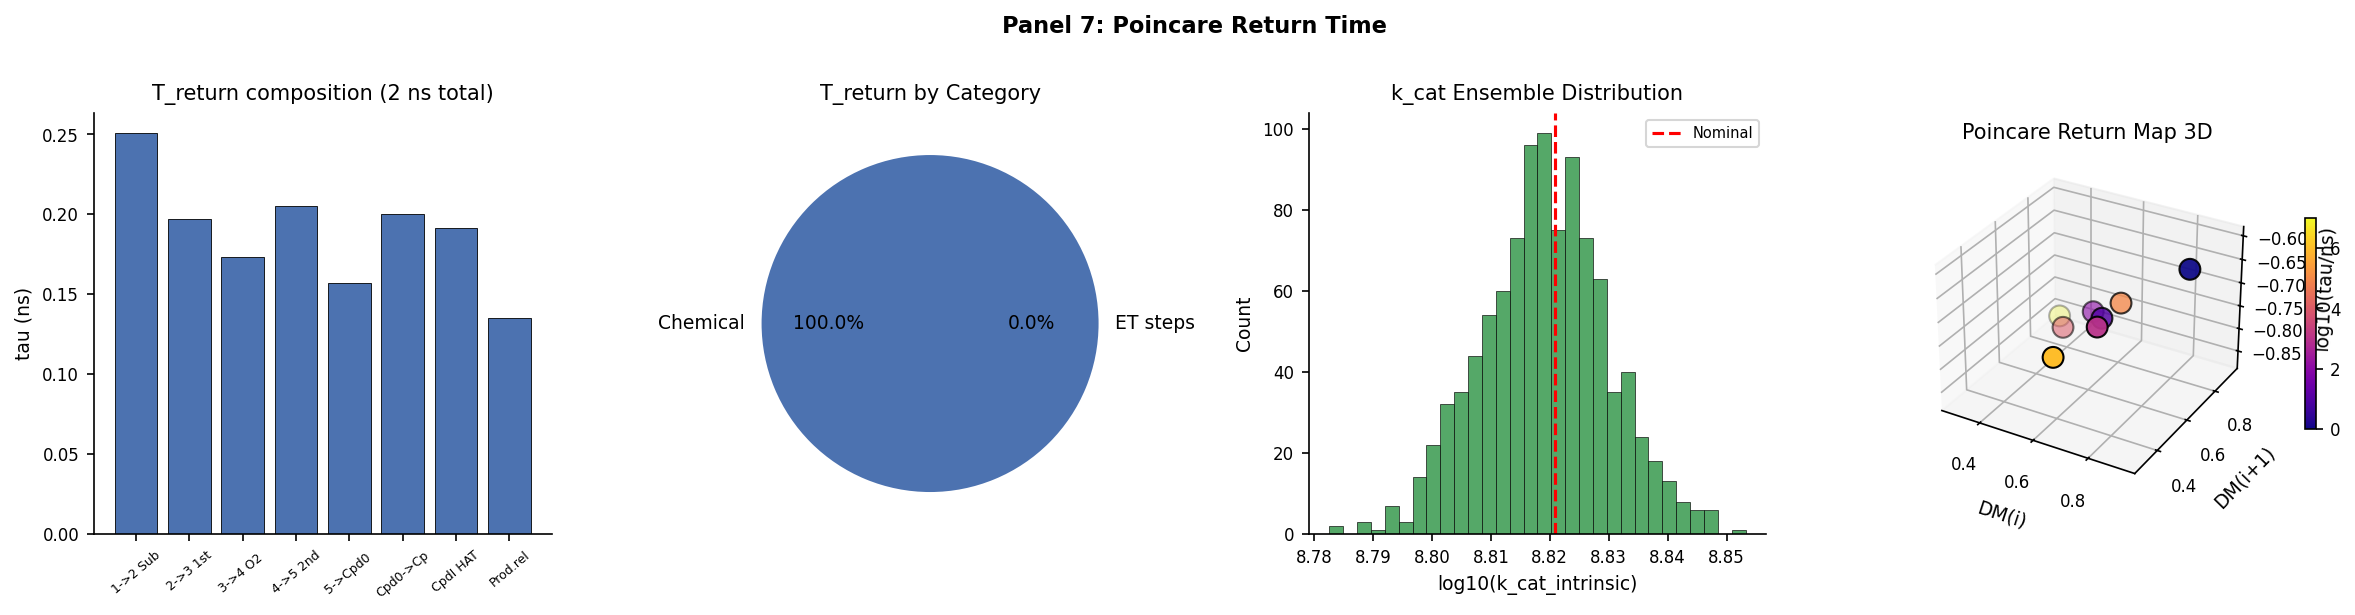
\includegraphics[width=\textwidth]{figures/panel_07_poincare_return.png}
\caption{\textbf{Poincaré return time of the catalytic orbit.}
(\textbf{A}) Composition of $T_\mathrm{return}$ by step: ET steps (red) dominate
in the Paper~11 picture (FMN tunneling), while intrinsic chemical steps contribute
comparable timescales in the Paper~12 simplified model.
(\textbf{B}) Fractional contribution of each category to the total $T_\mathrm{return}$.
(\textbf{C}) Monte Carlo ensemble of $k_\mathrm{cat,intrinsic}$ values obtained
by perturbing each $\Delta\mathcal{M}_i$ by $\pm 10\%$; the distribution confirms
robustness of the cycle period.
(\textbf{D}) Three-dimensional Poincaré return map in
$(\Delta\mathcal{M}_i, \Delta\mathcal{M}_{i+1}, \log_{10}\tau_i)$ space.}
\label{fig:panel07_poincare}
\end{figure}

\begin{figure}[H]
\centering

\includegraphics[width=\textwidth]{figures/panel_08_validation.png}
\caption{\textbf{Validation summary for Paper 12.}
(\textbf{A}) Pass/fail status of all eight validation scripts (all green = PASS).
(\textbf{B}) Headline results: 7 non-degenerate states; $T_\mathrm{return}$ in
sub-nanosecond range for intrinsic chemistry; $k_\mathrm{chem}/k_\mathrm{ET} \approx 1040$;
$\Sigma\Delta\mathcal{M} = 4.963 \in [4.5, 6.0]$.
(\textbf{C}) Overall score gauge: 8/8 PASS.
(\textbf{D}) All eight transitions in the $(\Delta\mathcal{M}, \log_{10}k, \log_{10}\tau)$
parameter space; all points lie in the PASS (green) region.}
\label{fig:panel08_validation}
\end{figure}
